% **************************************************
% Document Class Definition
% **************************************************
\documentclass[%
	paper=A4,					% paper size --> A4 is default in Germany
	twoside=true,				% onesite or twoside printing
	openright,					% doublepage cleaning ends up right side
	parskip=full,				% spacing value / method for paragraphs
	chapterprefix=true,			% prefix for chapter marks
	11pt,						% font size
	headings=normal,			% size of headings
	bibliography=totoc,			% include bib in toc
	listof=totoc,				% include listof entries in toc
	titlepage=on,				% own page for each title page
	captions=tableabove,		% display table captions above the float env
	draft=false,				% value for draft version
]{scrreprt}%

% **************************************************
% Debug LaTeX Information
% **************************************************
%\listfiles

% **************************************************
% Information and Commands for Reuse
% **************************************************
\newcommand{\thesisTitle}{Designing and Implementing a System for Passive User Feedback}
\newcommand{\thesisName}{Janis Krasemann}
\newcommand{\thesisSubject}{Master Thesis}
\newcommand{\thesisDate}{March 29, 2018}
\newcommand{\thesisVersion}{0.1}

\newcommand{\thesisFirstReviewer}{Dr. Simon Oberth\"ur}
\newcommand{\thesisFirstReviewerUniversity}{\protect{Paderborn University}}
\newcommand{\thesisFirstReviewerDepartment}{Software Innovation Campus Paderborn}

\newcommand{\thesisSecondReviewer}{John Doe}
\newcommand{\thesisSecondReviewerUniversity}{\protect{Paderborn University}}
\newcommand{\thesisSecondReviewerDepartment}{Software Innovation Campus Paderborn}

\newcommand{\thesisFirstSupervisor}{Bj\"orn Senft}
\newcommand{\thesisSecondSupervisor}{Dr. Simon Oberth\"ur}

\newcommand{\thesisUniversity}{\protect{Paderborn University}}
\newcommand{\thesisUniversityDepartment}{Faculty for Computer Science, Electrical Engineering and Mathematics}
\newcommand{\thesisUniversityInstitute}{Computer Science}
\newcommand{\thesisUniversityGroup}{Database and Information Systems}
\newcommand{\thesisUniversityCity}{Paderborn}
\newcommand{\thesisUniversityStreetAddress}{Warburger Stra{\ss}e 100}
\newcommand{\thesisUniversityPostalCode}{33098}

% **************************************************
% Load and Configure Packages
% **************************************************
\usepackage[utf8]{inputenc}		% defines file's character encoding
\usepackage[english]{babel} % babel system, adjust the language of the content
\usepackage[					% clean thesis style
	figuresep=colon,%
	sansserif=false,%
	hangfigurecaption=false,%
	hangsection=true,%
	hangsubsection=true,%
	colorize=full,%
	colortheme=bluemagenta,%
	bibsys=bibtex,%
	bibfile=bib-refs,%
	bibstyle=alphabetic,%
]{cleanthesis}
% JK Custom setup
\usepackage{todonotes}
\usepackage[printonlyused]{acronym}
% !TEX root = ./thesis.tex
%
\acrodef{CQRS}{Command Query Responsibility Segregation}
\acrodef{EDSD}{experiment-driven software development}
\acrodef{CSE}{Continuous Software Engineering}
\acrodef{REST}{Representational State Transfer}
\acrodef{SQL}{Structured Query Language}
\acrodef{CQL}{Cassandra Query Language}
\acrodef{DSL}{Domain Specific Language}
\acrodef{YAML}{YAML Ain't Markup Language}
\acrodef{VM}{Virtual Machine}
\acrodef{CLI}{Command Line Interface}
\acrodef{RSS}{Rich Site Summary}
\acrodef{API}{Application Programming Interface}
\acrodef{TCP}{Transmission Control Protocol}
\acrodef{UDP}{User Datagram Protocol}
\acrodef{HTTP}{Hypertext Transfer Protocol}
\acrodef{XHR}{XMLHttpRequest}
\acrodef{SPA}{Single-Page Application}
\acrodef{UX}{User Experience}
\acrodef{IFAS}{Implicit Feedback Analysis System}
\acrodef{HTML}{Hypertext Markup Language}
\acrodef{OSI}{Open Systems Interconnect}
\acrodef{JSON}{JavaScript Object Notation}

\usepackage[noabbrev]{cleveref}
\usepackage[toc,page]{appendix}
\usepackage{listings}
% Adds Cleveref support for Listing
\crefname{lstlisting}{listing}{listings}
\Crefname{lstlisting}{Listing}{Listings}

\hypersetup{					% setup the hyperref-package options
	pdftitle={\thesisTitle},	% 	- title (PDF meta)
	pdfsubject={\thesisSubject},% 	- subject (PDF meta)
	pdfauthor={\thesisName},	% 	- author (PDF meta)
	plainpages=false,			% 	-
	colorlinks=false,			% 	- colorize links?
	pdfborder={0 0 0},			% 	-
	breaklinks=true,			% 	- allow line break inside links
	bookmarksnumbered=true,		%
	bookmarksopen=true			%
}

% **************************************************
% Document CONTENT
% **************************************************
\begin{document}

% --------------------------
% rename document parts
% --------------------------
%\renewcaptionname{ngerman}{\figurename}{Abb.}
%\renewcaptionname{ngerman}{\tablename}{Tab.}
\renewcaptionname{english}{\figurename}{Fig.}
\renewcaptionname{english}{\tablename}{Tab.}

% --------------------------
% Front matter
% --------------------------
\pagenumbering{roman}			% roman page numbing (invisible for empty page style)
\pagestyle{empty}				% no header or footers
% !TEX root = ../thesis.tex
%
% ------------------------------------  --> cover title page
\begin{titlepage}
	\pdfbookmark[0]{Cover}{Cover}
	\flushright
	\hfill
	\vfill
	{\LARGE\thesisTitle \par}
	\rule[5pt]{\textwidth}{.4pt} \par
	{\Large\thesisName}
	\vfill
	\textit{\large\thesisDate}	
\end{titlepage}


% ------------------------------------  --> main title page
\begin{titlepage}
	\pdfbookmark[0]{Titlepage}{Titlepage}
	\tgherosfont
	\centering

	{\Large \thesisUniversity} \\[4mm]
	
\includegraphics[width=12cm]{gfx/UPB-Logo.png} \\[2mm]
	\textsf{\thesisUniversityDepartment} \\
	\textsf{\thesisUniversityInstitute} \\
	\textsf{\thesisUniversityGroup} \\

	\vfill
	{\large \thesisSubject} \\[5mm]
	{\LARGE \color{ctcolortitle}\textbf{\thesisTitle} \\[10mm]}
	{\Large \thesisName} \\

	\vfill
	\begin{minipage}[t]{.27\textwidth}
		\raggedleft
		\textit{1. Reviewer}
	\end{minipage}
	\hspace*{15pt}
	\begin{minipage}[t]{.65\textwidth}
		{\Large \thesisFirstReviewer} \\
	  	{\small \thesisFirstReviewerDepartment} \\[-1mm]
		{\small \thesisFirstReviewerUniversity}
	\end{minipage} \\[5mm]
	\begin{minipage}[t]{.27\textwidth}
		\raggedleft
		\textit{2. Reviewer}
	\end{minipage}
	\hspace*{15pt}
	\begin{minipage}[t]{.65\textwidth}
		{\Large \thesisSecondReviewer} \\
	  	{\small \thesisSecondReviewerDepartment} \\[-1mm]
		{\small \thesisSecondReviewerUniversity}
	\end{minipage} \\[10mm]
	\begin{minipage}[t]{.27\textwidth}
		\raggedleft
		\textit{Supervisors}
	\end{minipage}
	\hspace*{15pt}
	\begin{minipage}[t]{.65\textwidth}
		\thesisFirstSupervisor\ and \thesisSecondSupervisor
	\end{minipage} \\[10mm]

	\thesisDate \\

\end{titlepage}


% ------------------------------------  --> lower title back for single page layout
\hfill
\vfill
{
	\small
	\textbf{\thesisName} \\
	\textit{Designing and Implementing a System for Passive User Feedback} \\
	\thesisSubject, \thesisDate \\
	Reviewers: \thesisFirstReviewer\ and \thesisSecondReviewer \\
	Supervisors: \thesisFirstSupervisor\ \\[1.5em]
	\textbf{\thesisUniversity} \\
	\textit{\thesisUniversityGroup} \\
	\thesisUniversityInstitute \\
	\thesisUniversityDepartment \\
	\thesisUniversityStreetAddress \\
	\thesisUniversityPostalCode\ and \thesisUniversityCity
}
		% INCLUDE: all titlepages
\cleardoublepage

\pagestyle{plain}				% display just page numbers
% !TEX root = ../proposal.tex
%
\pdfbookmark[0]{Abstract}{Abstract}
\chapter*{Abstract}
\label{sec:abstract}
\vspace*{-10mm}

Because an increasing amount of computer engineers have been frustrated with failing software products due to the slow and inflexible phases of classical software engineering, alternative practices such as \emph{Continuous Software Engineering} have emerged and gained a lot of traction during the past decade.
In order to continuously improve a software system, reliable usage data from the user is needed.
%These experiments help the creators of a piece of software to test and validate their assumptions about a product and its features early in the development process.
%User feedback is the data upon which these experiments rely.
% What is the problem?
%The area of innovation via experimentation in the software industry is already well researched, but lacks a more holistic view on collecting, aggregating and analysing the passive user feedback needed for evaluating an experiment.
The area of Continuous Software Engineering is already well researched but lacks a more holistic view on collecting, aggregating and analyzing the user feedback needed for effectively improving the system.
%Why is this a problem?
%This is problematic because, although many companies realise the need for experimentation in their development process, they struggle with the systematic adoption of these practices.
This is problematic because, although many companies realize the need for continuity in their development process, they struggle with the systematic adoption of these practices.
%What is the / a solution?
By researching how to design and implement a system for establishing passive user feedback with considerably low effort, this thesis aims to fill this gap.
It is expected that event sourcing is a good fit for realizing such a system, which will be further investigated in the thesis.
%Event sourcing is a storage solution in which data is stored in the form of immutable event objects representing actions on business objects; in combination, all these events represent the application state.
Designing and implementing said system includes researching solutions for storing, aggregating and analyzing user feedback data.
A prototype using the chosen technologies is then implemented, which involves setting up and configuring various services as well as writing software that connects them.
The system is evaluated via a controlled experiment in order to validate the assumptions in this thesis.
%This will presumably involve either a user test for gathering passive user feedback, or analysing the user actions in an existing data set.
%The gathered data is then aggregated and analysed using the implemented system, and then compared with the results of a questionnaire with usability experts.
%Why is this a solution / what is ?
Practitioners in the software industry could use the system presented in the thesis as a reference for introducing collection and analysis of passive user feedback into their software, which facilitates the adoption of Continuous Software Engineering.
		% INCLUDE: the abstracts (english and german)
\cleardoublepage
%
%% !TEX root = ../thesis-example.tex
%
\pdfbookmark[0]{Acknowledgement}{Acknowledgement}
\chapter*{Acknowledgement}
\label{sec:acknowledgement}
\vspace*{-10mm}

\Blindtext[2][2]
 % INCLUDE: acknowledgement
%\cleardoublepage
%
\setcounter{tocdepth}{2}		% define depth of toc
\tableofcontents				% display table of contents
\cleardoublepage

% --------------------------
% Body matter
% --------------------------
\pagenumbering{arabic}			% arabic page numbering
\setcounter{page}{1}			% set page counter
\pagestyle{maincontentstyle} 	% fancy header and footer

% !TEX root = ../thesis.tex
%
\chapter{Introduction}
\label{ch:intro}

% CONTEXT

% GAP

% INNOVATION

% copy from proposal:

Best practices in software development changed dramatically since its origins in the 1950's~\cite{boehm2006view}.
Software engineering in most of the 20th century was largely based on careful planning and specification and therefore rather slow-paced and inflexible.
Since twenty years, however, these plan-driven development methods have been frustrating many people because the influencing circumstances change more and more rapidly, not least due to the growing importance of the internet~\cite{Williams2003}.
A result of this rapid change of the environment is that product features, which were perfectly valid at the time of their envisioning, became outdated, irrelevant or otherwise undesirable while the feature was still being planned or implemented -- not to mention features that are in fact not desired by the customers in the first place.
This insight is often not gained until the feature is shipped to the customer.
As a consequence, short release cycles and fast customer feedback have steadily been growing in importance.
These values are emphasized in \acf{CSE}~\cite{Bosch2014}, which adopts and extends the principles from \emph{DevOps} and agile software development~\cite{Fitzgerald2017,fowler2001agile}.

Adopting the core premises of \ac{CSE} is considered to be a gradual process, which is represented by the \emph{Stairway to Heaven}~\cite{Olsson2012} (see~\cref{fig:stairway}).
Starting from classical software development, the next step is agile software development.
This step is followed by continuous integration and deployment, respectively. 
The last step in the Stairway to Heaven is "Research \& Development as an Innovation System".
This means that the continuity gained in the previous steps is used for frequently deploying changes to the customers.
These changes are then assessed by analyzing user feedback data which was previously gathered using active or passive methods.
While active user feedback, e.g. in form of surveys, can yield useful qualitative observations about the product, the fact that the user has to actively take time for giving their feedback is often problematic.
Passive user feedback avoids this problem by automatically collecting feedback while the user works with the system; an example for this is measuring the time a user needs to perform certain actions in the software.
An \emph{evolutionary system} as described here allows for quicker responses to market changes and more accurate estimation of customer needs.

\begin{figure}[htb]
        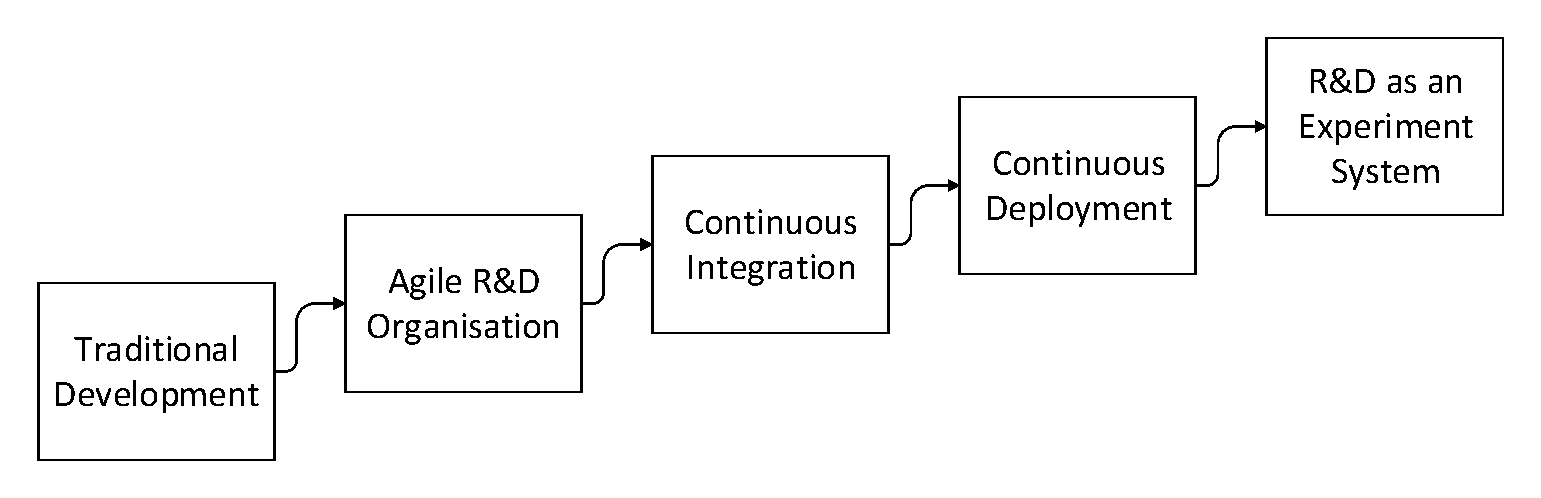
\includegraphics[width=\textwidth]{gfx/stairway.pdf}
        \caption{The "stairway to heaven" evolutionary model; adapted from~\cite{Olsson2012}.}
        \label{fig:stairway}
\end{figure}

%\cite{Bosch2014}

%The results of such an experiment are then used for deciding wether the feature should become a part of the final product.
%Thus, the goal in this case is to increase the effectiveness of developing a software product by implementing the \emph{right} features.
%Experiments are also used in order to compare different implementations of the same feature, thus improving the quality of an existing feature.
%This approach is contrary to the more classical software development methods, in which the stakeholders make certain assumptions which result in the envisioning of a feature, with feedback by a customer or stakeholder being given only much later in the development process~\cite{Bosch2012}.

%The core premise in innovation experiment systems is the continuous implementation and validation of assumptions about envisioned features via experiments in short sprints~\cite{Bosch2014}.
%The results of such an experiment are then used for deciding wether the feature should become a part of the final product.
%Thus, the goal in this case is to increase the effectiveness of developing a software product by implementing the \emph{right} features.
%Experiments are also used in order to compare different implementations of the same feature, thus improving the quality of an existing feature.
%This approach is contrary to the more classical software development methods, in which the stakeholders make certain assumptions which result in the envisioning of a feature, with feedback by a customer or stakeholder being given only much later in the development process~\cite{Bosch2012}.

The agile and continuous work methods in \ac{CSE} come with several implications for the system architecture and the company culture~\cite{Lindgren2015,Olsson2012}.
In particular, monolithic software systems are considered too cumbersome and slow to change; instead, small services that communicate with each other through a well defined but lightweight API are recommended.
\citet{ford2017building} argue that such distributed systems work well with the \emph{Parallel Model} concept introduced by \citet{WEB:Fowler:2005-2}.
The rationale is that using Parallel Model, services can work with their own specialized read model without interfering with or complicating the overall application state.
In order to make use of Parallel Model, it is recommended that the system also uses \emph{Event Sourcing}~\cite{WEB:Fowler:2005,WEB:Fowler:2005-2}.
Event sourcing is a storage solution in which data is stored in the form of immutable event objects representing actions on business objects; in combination, all these events represent the application state.
The most obvious advantage of this approach is that the event log represents a complete log of all transactions.
More importantly, however, this also allows for the execution of temporal queries which compute the application state at any given point in time, and the ability to replay events, possibly after modifying the application state at a certain point in time.
A consequence of event replayability is that events can be received in any given sequence, which otherwise is a common problem in asynchronous systems.

This thesis aims at taking a more holistic approach to the innovation system concept from \ac{CSE} by designing and implementing a system that allows for easy collection of passive user feedback (\cref{sec:intro:goals} describes the objectives in more detail).
The result will be a set of interacting services which provide the ability to collect, aggregate and analyze passive user feedback in order to facilitate innovation in the research and development process.
It is anticipated that this system will profit from the usage of even sourcing, but this has to be further investigated in the thesis.
The resulting system shall be called \ac{IFAS}.
It can be adopted by individuals and companies in the software industry who want to fully embrace \ac{CSE} and thus take the last step in the Stairway to Heaven.

% \cite{Bosch2012}: First, it is focused on continuously evolving the software by frequently deploying new versions. Second, customers and customer usage data play a central role throughout the development process. Third, development is focused on innovation and testing as many ideas as possible with customers to drive customer satisfaction and, consequently, revenue growth.

\section{Motivation}
\label{sec:intro:motivation}

TODO: explain that the developed system enables / improves: (cf. \cite{Bosch2012} figure 2) 

- AB testing, collecting metrics \& performance metrics (due to the functionality)

- can also be used in non-commercial deployment because of its flexibility and because its free!

- classify how the pre-dev, non-commercial and commercial deployment phases and the scopes (optimization, new features, new products) fit here

\begin{table}
\centering
\begin{tabular}{p{2.5cm}|p{3.2cm}p{3.2cm}p{3.2cm}}
 & \textbf{Pre-development} & \textbf{Non-commercial deployment} & \textbf{Commercial \newline deployment}  \\ \hline
Optimization & Ethnographic studies & Independently deployed extensions &\textit{ A/B testing}  \\
New features & Solution jams & Feature alpha & Instrumentation / \textit{collecting metrics}  \\
New products & Advertising\newline Mockups\newline BASES testing & Product alpha\newline Labs website & Surveys\newline Performance metrics 
\end{tabular}
\caption[The scope of innovation experiments by \citet{Bosch2012}.]{
The scope of innovation experiments by \citet{Bosch2012}.
\ac{IFAS}' functionality enables A/B testing and collecting metrics (\textit{italic}).
Because the system is free and due to its flexibility, it also potentially enables these for non-commercial deployments.
}
\end{table}

% Most techniques were based on eliciting direct customer feedback through familiar means such as stakeholder interviews and surveys, prototypes, usability and user experience testing, and other forms of user testing. Bug reports and feature voting were also used as a way to guide development. \cite{lindgren2015software}

% Focusing on products and features that create the most customer value was seen as a way to speed up development: ?I don?t think you can accelerate anything. What you can do is do less.? \cite{lindgren2015software}

%copy from proposal

The last step in the Stairway to Heaven of \acf{CSE} is introducing an innovation system, also referred to as an \emph{experiment system}~\cite{Olsson2012}.
Several companies have published their findings about experimentation in the software development process, in the form of scientific papers or blog posts.
Amongst others, Microsoft~\cite{Kohavi2013}, LinkedIn~\cite{Xu2015}, Google~\cite{Tang2010}, Facebook~\cite{Bakshy2014}, and Netflix~\cite{WEB:Netflix:2016} issued reports about best practices and pitfalls that they experienced, all concluding that introducing experimentation into the software development process benefits both the choice about which features to implement as well as their quality.
In addition, several authors have published scientific papers in which they propose models and architectures for experimental software development~\cite{Fagerholm2014,Fagerholm2017,Johanssen2017,Lindgren2015}.
Although practitioners in the software industry often claim that they embrace experimentation and innovation in their research and development process, these practices are still not fully adopted according to a study by \citet{lindgren2015software}.
Especially the systematic and continuous aspects of experimentation lack adoption.

% Problem f�r Motivation ist hier: Wenn ich nicht direkt auf Event Sourcing Bezug nehme (d.h. es offen lasse ob Event Sourcing verwendet wird oder nicht) wird der Scope zu gro�: "Wie kann an eine Experimentier-Plattform implementieren" haben andere Leute schon beantwortet.
While the overall area of experimentation in software development is thus well researched, most papers are either more of a report about specific best practices or a rather abstract description of an architecture.
The same applies to the paper that initially proposed the Stairway to Heaven concept~\cite{Olsson2012}.
This is problematic for potential applicants of \ac{CSE}, because while these reports are very practice-oriented, they lack a more general view on the problem at hand, and the other way around for the architecture-focused papers.
Therefore, the aim of this thesis is to bridge this gap and provide a more holistic view on collecting, aggregating and analyzing passive user feedback.
This will enable applicants to implement their own innovation / experiment systems as described in \ac{CSE}, based on a scientifically tested architecture.


\section{Objectives}
\label{sec:intro:objectives}

% copy from proposal

The goal of the thesis is to design, implement and validate a system for passive user feedback with a more holistic view of the problem than in existing publications.
Using this system, it shall be possible to visualize and analyze passive user feedback that was previously supplied to its storage layer.
In order to accomplish this task, a system with functionalities as pictured in \cref{fig:system:vision} has to be implemented.
The concrete objectives are as follows:

\begin{enumerate}
\item Classify existing solutions and approaches for establishing passive user feedback.
\item Design and implement a system that allows the collection of passive user feedback with considerably low effort.
This part of the system is comprised of the storage layer, an aggregation service and a hypothetical client application which logs events to storage whenever the user performs certain actions (cf. 4.).
%It also features two users: The end user of the client application, and the analyst who wants to evaluate the user feedback.
These events can be purely UI related, such as click or hover events, but can also be related to the business logic, like executing transactions or creating content.
In order to forward the user feedback data to the analysis application (cf. 3.), the aggregation service has to fetch the appropriate data from the store.
While making use of a caching mechanism during this step would certainly make sense, such a feature will presumably not be part of the final solution due to the additional complexity; if this is the case, the system shall be easily extensible for introducing such a feature.
This objective involves researching and assessing fitting infrastructure and tooling solutions.
\item Design and implement this system such that it also allows analysis of collected user feedback.
Feedback should be ready for analysis within at most a minute.
When someone wants to evaluate the collected user feedback via the analysis application, the application shall display the corresponding data in an appropriate format, which it fetches from the aggregation service.
The best approach for displaying the data has yet to be evaluated but will involve some graphical representation in form of charts and/or graphs.
This objective also implicates research and choosing of appropriate solutions that shall be used for this part of the system.
\item Evaluate how this system performs, which involves collecting user feedback and analyzing it.
Implementation of the client application itself will not be done for the purpose of this thesis.
Instead, some existing application shall be extended in order to log the appropriate events or an existing data set such as the one presented by \citet{Deka:2017:Rico} shall be used.
In the latter case, some application or script has to be written which imports the needed UI interaction data to the database.
\item As an additional requirement, the developed system shall be platform independent, i.e. run on the most widely used operating systems Linux, MacOS, and Windows.
\end{enumerate}

\begin{figure}[htb]
        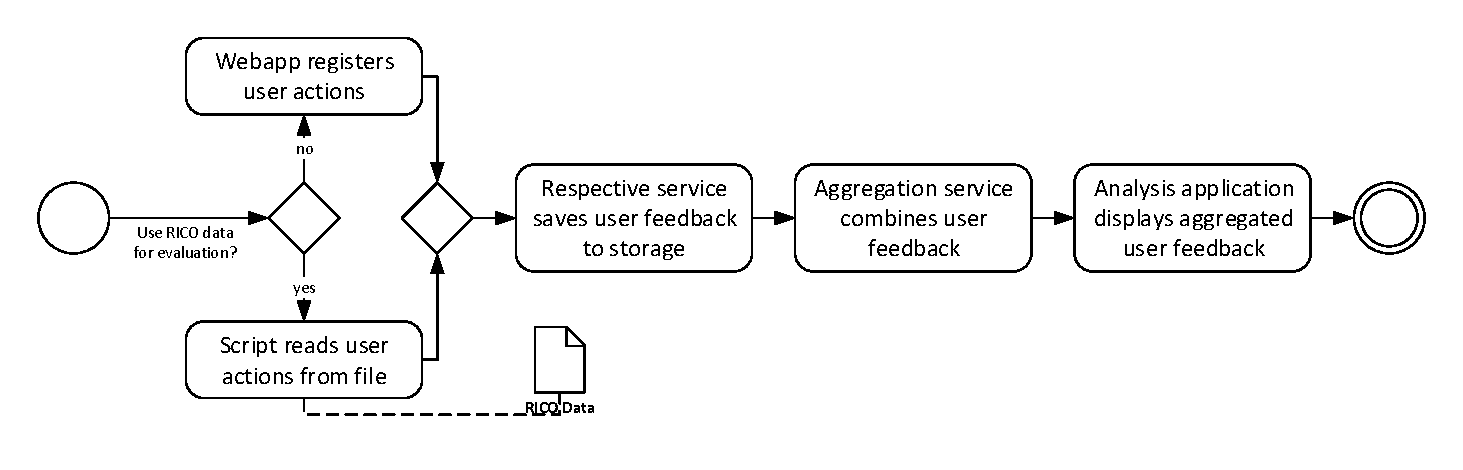
\includegraphics[width=1.1\textwidth]{gfx/architecture-3.pdf}
        \caption{The activities that the envisioned system is able to perform.}
        \label{fig:system:vision}
\end{figure}

%\section{Motivation and Problem Statement}
%\label{sec:intro:motivation}

\section{Approach}
\label{sec:intro:approach}

% copy from proposal

In order to achieve the objectives described in \cref{sec:intro:goals}, the working time of the thesis will roughly be divided into three segments: Research, implementation, and evaluation.
Putting the gained findings into writing is part of each of these segments.

Part of the research phase will be dedicated to reading up on the central topics for this thesis, namely but not exclusively \acf{CSE}, event sourcing, \acf{CQRS} and passive user feedback as well as methods for collecting it.
Aside from that, some decisions regarding the architecture and technology require additional research.
This involves researching, comparing and finally choosing an appropriate storage solution.
Current findings suggest that an event store, and in particular the Event Store reference implementation\footnote{\url{https://eventstore.org/}}, is a good fit for this.
The advantages of using event sourcing in this context are as follows:

\begin{enumerate}
\item Event replayability could be used to further mitigate the risk of creating experimental features: If a change in the software causes some faulty event to be created, it can later be modified or deleted.
Incorrect changes that are based on this faulty event can automatically be corrected using the Retroactive Event technique~\cite{WEB:Fowler:2005-3}.
Contrary to classical relational databases, the overall application state in an event store would not be corrupted by this.
It would also be possible to create separate event stores just for specific features, which could later be applied to the main event store by replaying the events from the experimental store.
\item When a feature has to be analyzed, temporal queries could be used for retrieving all events in a specific time frame.
\item Event sourcing and \ac{CQRS} advocate a distributed system architecture -- which is also true for the evolutionary systems present in \ac{CSE}~\cite{ford2017building}.
\end{enumerate}

In particular, the temporal query feature could render additional aggregation services obsolete.
Additional backup systems that roll back changes issued by potential experiments could also possibly be removed because of an event stores inherent ability to roll back and redo changes.
These assumptions would have to be validated over the course of the actual thesis.

A solution for aggregating the data has to be researched; the aforementioned temporal query feature is one candidate for this, another is Elasticsearch\footnote{\url{https://www.elastic.co/}}.
This aggregation service has to be paired with some service or application that analyses the generated data; Kibana\footnote{\url{https://www.elastic.co/products/kibana/}} seems to be a promising solution.
In order to achieve high platform independence and flexibility, a container platform such as Docker\footnote{\url{https://www.docker.com/}} will be used which also requires some research.
In order to be able to decide whether to use the RICO dataset~\cite{Deka:2017:Rico} instead of a custom client application for the evaluation part, this dataset will have to be assessed further.

The first task in the implementation phase will be to finalize the system architecture.
While the architecture is not expected to be overly complex and the first draft of its capabilities already exists at the time of writing (cf. \cref{fig:system:vision}), some alterations are possible and expected.
This task also involves deciding which data to save to the storage layer and which logical structure this data has to have.
When the system architecture design is finalized, the actual implementation can begin, which first of all involves setting up and configuring the storage solution.
If user feedback data is to be generated from a client application and not using the RICO dataset, the actual feedback logging has to be implemented as well.
Depending on the choice of aggregation service, if any, this service also has to be set up and/or implemented; the same holds for the analysis solution.

Finally, the implemented solution will be evaluated by executing up to two experiments.
The first experiment for the evaluation will be a questionnaire in which usability experts answer questions about a given application.
The results of the questionnaire will be compared to the passive user feedback data of the given application.
Depending on the means of collecting this user data, an experiment for collecting this data has to be designed and executed with some test subjects; this is not necessary if the RICO dataset is chosen as the source of user data.
The experiments have to be planned and executed carefully in order to have high internal and external validity~\cite{Huitt2010}.
Existing studies about best practices and pitfalls of running controlled experiments can be useful here~\cite{Kohavi2009}.


\section{Thesis Structure}
\label{sec:intro:structure}

\todo{Paragraphen zusammenziehen oder mehr schreiben}

In the fundamentals (\ref{ch:fundamentals}), the topics that are required to understand the contents of this thesis are explained.

The related work chapter (\ref{ch:related-work}) deals with scientific papers which have already explored the topics of passive user feedback and \ac{CSE} to some degree.

The first step to doing the design and implementation of the passive feedback system was to explore, evaluate and classify existing solutions for data storage, aggregation and analysis.
This is described in the Classifications chapter (\ref{ch:classifications}).

After choosing the technology for the implementation, various design decisions had to be made, which are explained in the System Design chapter (\ref{ch:design}).

The actual implementation details are then described in the subsequent chapter (\ref{ch:implementation}).

Upon finishing the implementation, the system was evaluated by a user and an expert survey, the methods and results of which are explained in the evaluation chapter (\ref{ch:evaluation}).

Possibilities for future work are given in its own chapter (\ref{ch:future-work}), followed by the conclusion (\ref{ch:conclusion}).

The appendix contains source code and configuration files of the various applications and services that were implemented and used.
 % INCLUDE: introduction
% !TEX root = ../thesis.tex
%
\chapter{Fundamentals}
\label{ch:fundamentals}

[insert fluff piece about fundamentals here]

\section{Experiment-driven Software Development}
\label{sec:fundamentals:edsd}

\cite{Olsson2012}

\section{Implicit User Feedback}
\label{sec:fundamentals:implicit}

\cite{Kelly:2003:IFI:959258.959260}

Gathering implicit user feedback via eye tracking software is a valid alternative to using clickthrough data, but is not considered in this thesis for two reasons.
First, requiring an eye tracker for gathering implicit user feedback of generic web applications would be impractical.
Second, cursor movement was shown to be a good approximation of where the user's gaze is located~\cite{Huang2011}, thus it is expected that using an eye tracker would not yield significant additional in the given context anyway.

\section{Continuous experimentation surveys}
\label{sec:related:surveys}

\cite{lindgren2015software}

\cite{Bosch2012}

\cite{Gutbrod2017}

\section{Controlled Experiments}
\label{sec:fundamentals:experiments}

The earliest controlled experiment dates back to the 1700s, where the crew of a British ship suffered from scurvy, a common suffering that sailors tend to experience when exposed to a limited diet like on sea ships during that time.
As the ship was charging citrus fruits, the captain of the ship decided to do an experiment: 50\% of his sailors, the \emph{treatment} group, had limes added to their diet.
The other half of the crew did not eat any citrus fruits; these were the \emph{control} group.
Although the reasons were not known during that moment, the experiment was a success: The treatment group got better, and eventually all sailors had citrus fruits added to their diet~\cite{rossi2003evaluation,marks2000progress}.

This anecdote is an example for the simplest type of controlled experiment, in which users are randomly assigned to either the control or the treatment group.
While the treatment group is treated with the new version of the system that is being tested, the control group experiences the same system as before, without the modification.
Thus, each group contains 50\% of the user base, and the results of the control group can be used in order to control wether the treatment had any statistically significant effect~\cite{Kohavi2009}.
\todo{not enough about controlled experiments}
%The test that detects wether two variants are statistically different is called the \emph{null hypothesis}.
% more details in Kohavi2009

\section{Event sourcing}
\label{sec:fundamentals:event}

%abstract: what is event sourcing
The core premise of event sourcing~\cite{WEB:Fowler:2005} is that all changes to the application state are stored as immutable events, in the order in which they occur.
In aggregation, these events represent the whole application state.
%, contrary to classical relational databases,
\citet{Overeem2017} and \citet{Erb2016} have done some research on event sourcing and \citet{evans2004domain} grazes the topic in his book, stating that event sourcing is useful for X.
Apart from these few examples, literature in form of books or scientific papers regarding event sourcing is rather rare.
Several extensive blog posts by \citet{WEB:Fowler:2005} and \citet{young2010whyeventsourcing} explain the concepts and methods in great extensive though.
\todo{vertiefen}

Inherent to event sourcing is the lack of an explicit schema, just as in NoSQL databases~\cite{fowler2013schemaless}.
Instead, the schema is represented implicitly within the application itself.
This enables more flexibility, as any type of data can be saved in storage without defining a schema first.
However, it also comes with some drawbacks, especially when this implicit schema changes; \citet{Overeem2017} investigate these.
\ac{IFAS} assumes that the implicit schema is not changed after its initial launch.

\subsection{Features}

% what can you do with event sourcing: aggregation, rollback
When all changes to the application state are introduced via event objects, various capabilities arise which are not possible if only the application state is stored.
As \citet{WEB:Fowler:2005} describes, these are Complete Rebuild, Temporal Query, and Event Replay:

\begin{description}
\item [Complete Rebuild]
The application state can be discarded and then rebuilt by querying all events that occurred since the beginning.
\item [Temporal Query]
Instead of doing a complete rebuild up to the present application state, the rebuild can also be done to a given date somewhere in the past.
By doing so, the application state at the given point in time is re-created.
\item [Event Replay]
In another variant of the complete rebuild, it is also possible to change a certain past event and then replay all subsequent events, which yields a variant of the current application state reflecting the consequences introduced by the modified event.
This can be done just for testing purposes, for correcting a wrong event or for fixing errors caused by events occurring in the wrong order.
\item [Reversing Events]
If the events are designed according to [...] it is possible to undo a given event by creating its reverse version.
This is easy if the event encodes the difference between the occurring event and the application state at that point, for example for events that add or subtract a numeral value.
Reversing of events is not that straightforward if this difference approach is not used -- the events should include the previous and updated value in that case, but this is not ideal in every case.
It is important to note that event reversability can also be achieved by reverting to a given snapshot of the application state and then replaying all events \emph{except} the event that shall be undone.
\item [Delayed Application]
% or whatever it is called
\end{description}

A well known example for a system which makes use of event sourcing techniques is the version control system Git\footnote{\url{http://git-scm.com/}}.
It does complete rebuilds when a project is checked out for the first time and uses temporal queries for introducing changes when switching to an existing branch. \todo{check if this is really how Git does this}

% what can you NOT do / disadvantages
Aside from its advantages, event sourcing is not an ideal storage solution for all use cases.
First of all, event sourcing introduces a level of indirection to the application, which makes the system architecture more complicated.
Additionally, as this is an altogether different concept than storing the state directly in a database, it is thus hard to grasp and thoroughly understand for most developers.
% External Updates
% External Queries

% What about code changes?

% how some of these disadvantages can be worked around (short)
As events are immutable, event sourcing does not have a delete operation, because immutability prohibits deletion.
It is however possible to create explicit removal events -- for example a \texttt{CustomerRemoved} event for deleting a customer -- which in the end results in an application state where the item in question is not present anymore.

\cite{WEB:Fowler:2011}


\subsection{Subscriptions}

Subscriptions are a mechanic that allow clients to be notified when new events are written to a stream.
There are three types of subscriptions:

\begin{description}
\item[Volatile Subscription]
The time at which the subscription is enabled is considered as its starting point.
All events that are written \emph{after} the starting point are considered by the subscription; prior events are ignored.
\item[Catch-Up Subscription]
This subscriptions allows the starting point to be supplied as a parameter by the client, e.g. in form of an event number.
Events that were written after the given starting point are served immediately to the client.
The catch-up subscription behaves just as the volatile subscription for all subsequently written events.
\item[Persistent Subscription] 
This is a special kind of catch-up subscription.
The persistent subscription stores the subscription state on the server side and supports the \emph{competing consumers} messaging pattern\footnote{\url{https://docs.microsoft.com/en-us/azure/architecture/patterns/competing-consumers}}.
This pattern stipulates multiple consumers which asynchronously and independently handle messages generated by the server.
It is not relevant which of the services handle a specific message, as each behaves identically, and every message is guaranteed to be delivered \emph{at least once}.
Therefore, it is possible to set up multiple worker services for feeding event store data into a consuming service and thus enable horizontal scalability.
\end{description}

\section{Evaluation Fundamentals}
\label{sec:fundamentals:evaluation}

ISTQB fundamental testing process~\cite{graham2008foundations}
Dwell Time(?)~\cite{Liu2010}\cite{Kim2014}

\section{Docker}
\label{sec:fundamentals:docker}

Docker\footnote{\url{https://www.docker.com}} is a container platform that allows for lightweight and flexible virtualization of services and applications.
The central concept of Docker are its containers, which package application code as well as dependent libraries, binaries, and settings.
It is important to note that a Docker container does not contain a host operating system -- a main difference between a container and a \ac{VM}.
This makes containers more lightweight than \ac{VM}s, resulting in a smaller footprint in terms of CPU usage, main memory and storage.
A container is executed by the Docker engine, which is available for all modern operating systems such as Linux, Windows and MacOS.

Docker containers are defined by a \emph{Dockerfile}, which hosts a set of instructions that tell the Docker engine how to build the image which in the end is instantiated in a container (\cref{code:fundamentals:docker:dockerfile} shows an exemplary Dockerfile).
Each instruction of the Dockerfile creates another filesystem layer, which in combination produce the final image.
In this case, the Dockerfile states that the base image shall be the \texttt{nginx} image with version \texttt{1.13}; this creates the first image layer.
The \texttt{COPY} instruction copies the contents of the folder where the Dockerfile resides into the stated destination in the target filesystem, such that the copied files can be served by the NGINX instance; this creates the second image layer.
It is very important to note that the Docker engine saves image layers as diffs, meaning that a layer is described by its  difference with the layer below.
This results in high reusability of image layers: When the \texttt{COPY} instruction in the example Dockerfile is changed, only the second image layer has to be rebuilt, allowing for much faster build times.
%This suffices to bootstrap the containers itself, but in most cases additional configuration files are loaded into the container via volumes.

\lstinputlisting[label={code:fundamentals:docker:dockerfile},caption={Example Dockerfile}]{sourcecode/Dockerfile.txt}

Containers can be created and run via the Docker \ac{CLI}.
For example, the NGINX image previously described in \cref{code:fundamentals:docker:dockerfile} would first be containerized and then executed via the instructions given in \cref{code:fundamentals:docker:cli}.
The \texttt{-p} option specifies that the container's port 80 shall be exposed as port 8000 on the host operating system.

\lstinputlisting[label={code:fundamentals:docker:cli},caption={Build and run the NGINX example container via the Docker CLI},language=bash]{sourcecode/docker-cli.sh}

However, building and running images and containers via the Docker \ac{CLI} becomes tedious when a combination of multiple containers has to be managed.
\emph{Docker Compose} facilitates container composition by storing these build and run definitions in a single configuration file, using the data serialization language \ac{YAML}.
\Cref{code:fundamentals:docker:compose-yml} shows an exemplary \texttt{docker-compose.yml} file, which specifies that  the previously shown Dockerfile shall be used for building the image as a service called \texttt{server}, and that again port 8000 shall be exposed.
The image is then built, and the container subsequently run, via two commands as shown in \cref{code:fundamentals:docker:compose-run}.
While the approach using the Docker CLI may seem more concise in this limited example, Compose's advantages when combining multiple interconnected services become apparent when doing more complex container composition (cf. \cref{sec:implementation:orchestration}).

\lstinputlisting[label={code:fundamentals:docker:compose-yml},caption={Example docker-compose.yml}]{sourcecode/docker-compose-example.yml}
\lstinputlisting[label={code:fundamentals:docker:compose-run},caption={Build and run the NGINX example container via Compose},language=bash]{sourcecode/run-via-compose.sh}

The container architecture of Docker solves two challenges when creating distributed systems: application independence and bridging the development-operations gap.
Application independence is achieved by running every application in its own container which can only interact with other containers via explicitly defined interfaces (e.g. HTTP).
Secondly, Docker facilitates bridging the gap between the developers and operations teams, as the environment that the application is executed in -- the Docker container -- does not change between the development and production stages.
This makes Docker a popular technology for implementing DevOps.

Instead of Docker, a lot of alternative technologies could have been chosen as the virtualization solution.
These alternatives include services such as Vagrant, Kubernetes and Apache Mesos, some of which make use of Docker internally.
Docker was favored over the alternatives because of its maturity, good documentation, and my previous experiences with it, making this a partly subjective decision.
It would also be possible to run the passive user feedback system natively on a server or multiple servers, but this would have introduced unnecessary complications. % INCLUDE: fundamentals
% !TEX root = ../thesis-example.tex
%
\chapter{Related Work}
\label{sec:related}

\cleanchapterquote{A picture is worth a thousand words. An interface is worth a thousand pictures.}{Ben Shneiderman}{(Professor for Computer Science)}

\Blindtext[2][1]

\section{Related Work Section 1}
\label{sec:related:sec1}

\Blindtext[2][2]

\section{Related Work Section 2}
\label{sec:related:sec2}

\Blindtext[3][2]

\section{Related Work Section 3}
\label{sec:related:sec3}

\Blindtext[4][2]

\section{Conclusion}
\label{sec:related:conclusion}

\Blindtext[2][1]
 % INCLUDE: related work
% !TEX root = ../thesis.tex
%
\chapter{Assessment of Software Solutions}
\label{ch:classifications}

This chapter examines the various possible software solutions for the different parts of the \acf{IFAS}.
These parts are data storage, data aggregation, and data analysis, as described in \cref{sec:intro:objectives}.
This chapter also contains considerations about the choice of data source and about container orchestration (cf. \cref{sec:design:data-source,sec:classification:orchestration}).

Using the objectives described in the introduction (cf. \cref{sec:intro:objectives}) as a starting point, more concrete and fine grained requirements for each part of \ac{IFAS} were created.
These are listed at the beginning of each section.
Afterwards, possible software solutions are listed and then the evaluation part describes to which extent each software solution fulfills these requirements.

Following the initial motivation for this thesis (cf. \cref{sec:intro:motivation}), the architecture of \ac{IFAS} was envisioned with the principles of evolutionary architectures in mind.
For this reason, \ac{IFAS} follows a microservice approach for its architecture: The storage, aggregation, and analysis capabilities shall be provided by separate microservices instead of one monolithic application.
This makes the architecture more open to future, incremental change, which is the main reason behind applying an evolutionary architecture (cf. \cref{sec:fundamentals:evolutionary}).

\section{Data Storage Solutions}
\label{sec:classifications:storage}

The first technical decision was about the storage solution.
First, the requirements which the solution has to fulfill are explained, then the candidates are presented and evaluated according to these requirements in order to find the most appropriate solution.
The result is that Event Store is the most qualified solution for the storage requirements.

\subsection{Requirements}
\label{subsec:classifications:storage:req}

In accordance to the previously defined objectives for \ac{IFAS}, the data storage solution should offer scalable database capabilities for the connected application.
It should be possible to reuse the main storage of the application that \ac{IFAS} is added to if the same software is used.
Alternatively, \ac{IFAS}'s storage can be used in addition to an existing database.

\ac{CSE} requires the storage layer of such a system to have certain capabilities, namely flexibility and scalability.
%In addition to basic storage capabilities, the storage solution has to provide some functionalities related to the use case, such as temporal queries.
The following requirements for the storage solution were identified, based on which the candidates will be evaluated:

\begin{description}
\item [Basic storage capabilities]
The storage solution must at least provide means of creating and reading persisted data records.
\item [Modify]
In order to facilitate experimentation, the storage solution shall have some means of correcting faulty data records, i.e. an update and delete mechanic.
This is desirable in cases where a change in the software introduced erroneous behavior which has to be undone.
%It would not be sufficient to just spin up a separate instance of the storage solution for the experiment because users should not be aware of whether they are part of the treatment group.
\item [Cascading update (optional)]
In addition to a regular modify feature, the storage solution ideally also has some means of correcting all data that is invalid due to being dependent on one invalid data record.
This could be especially usable when a series of events initiated by the user is dependent on each other.
%\item [Temporal queries]
%It would presumably be useful to be able to retrieve all data records that were created within a specific time frame via some query.
%These queries have to be efficient because running an analysis must not affect the storage solution's normal operation performance.
%\todo{would this even be used with an aggregation service???}
%\todo{do not call this "temporal queries" as the event store already has a concept with that name}
\item [Scalability]
For performance reasons, the storage solution shall be vertically scalable, i.e. scale \emph{up} when a node that the service runs on is assigned more computing power.
The storage solution shall also be able to scale horizontally, i.e. scale \emph{out}, which means that it is able to increase its performance by adding more computing nodes to the network.
This is often solved via \emph{sharding}, where the data is split over multiple logical or physical storage instances, each of them shouldering a portion of the cumulative system load in a divide and conquer approach.
%Database clustering is done for various reasons. Clusters can improve availability, fault tolerance, and increase performance by applying a divide and conquer approach as work is distributed over many machines. Clustering is sometimes combined with partitioning and sharding to further break up a large complex task into smaller, more manageable units. 
\item [HTTP interface]
The storage solution shall have a \ac{HTTP} interface, therefore allowing other services and applications to store and retrieve data via a universally supported interface.
As most solutions considered in this chapter do indeed offer a \ac{HTTP} interface, this is the most straightforward way of connecting the different services and applications.
\ac{HTTP} may have worse performance than protocols operating on lower levels in the \ac{OSI} stack~\cite{zimmermann1980osi}.
Examples for such protocols are the \ac{TCP} and the \ac{UDP}, but the advantages in terms of flexibility make \ac{HTTP} the favored solution.
In cases where performance is critical, TCP could still be used if supported.
It should be noted that almost any storage solution can be extended to have an \ac{HTTP} interface by writing a wrapper in a general purpose programming language that exposes the database functionality.
However, this introduces additional implementation and communication overhead, as the database wrapper would have to be implemented manually -- not to mention potential security issues.
\item [Hosting]
\ac{IFAS} is planned to run on a Docker machine.
Thus, all services have to support this and in particular should not exclusively be \ac{SaaS} running on the respective company's servers.
This is beneficial in terms of platform independence and also regarding data protection, as running \ac{IFAS} as a \ac{SaaS} would mean potentially giving the company running the service access to the accumulated user feedback data.
\item [Free License]
The designed system shall be as widely applicable as possible and therefore not impose any financial requirements on the potential adopter.
Thus, the storage solution shall be available free for commercial use, e.g. in form of an open source license such as the GNU GPL\footnote{\url{https://www.gnu.org/licenses/gpl.html}} or Apache License\footnote{\url{https://www.apache.org/licenses/}}.
No rating is applied to the various open source licenses, especially in terms of how permissive they are.
Instead, such an evaluation is left at the discretion of the respective adopters of \ac{IFAS}, should they potentially have a problem with licenses such as the more permissive 2-Clause BSD License\footnote{\url{https://opensource.org/licenses/BSD-2-Clause}}.
\end{description}

%I additionally rate storage solution candidates based on maturity, licensing, and applicability.
%Maturity is a rather subjective metric but can be based at least partly on the technology's age and its popularity.
%Licensing could be an issue if the technology has a proprietary license, or if modifications have to be made to the source code (although the latter case is rather unlikely).
%Applicability refers to how well the technology is presumed to fit to the use case of storing, accessing and modifying multiple related user actions.
%\todo{Be more specific - which scale?}

\subsection{Candidates}

The possible data storage solutions are split into two main categories: \ac{SQL} databases and \ac{NoSQL} databases.
While there is conceptually no big difference between the different \ac{SQL} databases, the \ac{NoSQL} databases are further split into subcategories: Key-value stores, document stores, graph databases, and column databases.

As \citet{strauch2011nosql} describe, document stores have a rather simple data model compared to \ac{SQL} databases:
Data is stored in form of documents, which consist of key-value pairs.
Key-value stores are even simpler, as they do not have a notion such as documents and instead store all data as pairs of keys and values.
Column-oriented databases on the other hand save data in a more structured way, but store and process it column-oriented instead of row-oriented (as \ac{SQL} databases do).
Graph databases, as described by \citet{miller2013graph}, are very useful for specific use cases, especially in the field of chemistry and biology.
They store data according to graph theory, in the form of edges and nodes, which is beneficial if the stored data is highly connected.
In a classification of \ac{NoSQL} databases, \citet{popescu2010nosql} claims that graph databases are more complex than column databases or key-value stores, but offer more functionality in the form of graph theory.

The chosen databases in the \ac{SQL} category and in the subcategories of \ac{NoSQL} are constrained to a few of the most commonly used databases.
As the databases of each group in general have identical or at least very similar properties, the specific choice of representative is not expected to have a relevant impact.
One exception of this assumption are the document stores, where both Event Store and MongoDb are listed.
The candidates are:

\begin{itemize}[noitemsep]
\item \ac{SQL} Databases
\begin{itemize}[noitemsep]
\item Postgres
\item MySQL
\item MS-SQL
\item Oracle
\end{itemize}
\item NoSQL Databases
\begin{itemize}[noitemsep]
\item Document stores: Event Store, MongoDb
\item Graph databases: Neo4j
\item Key-value stores: Apache Ignite
\item Column databases: Cassandra
\end{itemize}
\end{itemize}

\subsection{Evaluation}

By analyzing each of the candidates, Event Store was determined to be the most appropriate solution, Neo4j and MongoDb being the most promising alternatives.
Other solutions came short in at least one integral requirement.
See \cref{table:classifications:storage} for a summary of the analysis.
As scalability is hard to grade on an absolute scale without doing time-expensive benchmarks, this requirement is not explicitly listed in the table.
Instead, the table states whether the solution in general supports clustering which is an indicator of good scalability capabilities; each solution's scalability is reasoned about in their respective passages in the textual evaluations.

\begin{table}[t]
\centering
\caption[Classification of storage solutions]{Classification of storage solutions; the requirements regarding basic storage capabilities and modifying data are not listed because all solutions satisfy these.}
\makebox[\textwidth][c]{
\begin{tabular}{l|l|l|l|l|l}
\textbf{Name} & \textbf{Type} & \textbf{Casc. Updates} & \textbf{Clustering} & \textbf{HTTP} & \textbf{License} \\ \hline
Event Store & Document & yes & yes & yes & BSD \\
Postgres & SQL & no & no & no & PostgreSQL \\
MySQL & SQL & no & yes & no & GPL / Proprietary \\
Oracle & SQL & no & yes & with addons & Proprietary \\
MongoDB & Document & no & yes & yes & GNU AGPLv3 \\
Ignite & Key-Value & no & yes & yes & Apache v2 \\
Neo4j & Document & yes & no & yes & GPL / Proprietary \\
Cassandra & Column & no & yes & no & Apache v2
\end{tabular}
}
\label{table:classifications:storage}
\end{table}

Using event sourcing as the technique for storing passive user feedback is a natural fit because the use case benefits greatly from the fact that not only the current state is saved, but also how this state was reached.
By storing the events that occur when a user uses the respective application, the complete interaction trace can be computed just by querying the event store.
Modification of the application state in general can be done simply by issuing a new event that reflects this change (e.g. an \texttt{AddressChangedEvent} if a customer's address shall be modified).
If other changes are dependent on this change, it is also possible to make use of the event replay technique by modifying the event that introduced the erroneous change and then replaying all subsequent events.
Event replayability could also be used to further mitigate the risk of creating experimental features: If a change in the software causes some faulty event to be created, it can later be modified or deleted.
Incorrect changes that are based on this faulty event can automatically be corrected using the Retroactive Event technique~\cite{WEB:Fowler:2005-3}.
Contrary to classical relational databases, the overall application state in an event store would not be corrupted by this.
Event Store supports multi-node clusters which replicate all written data from the master node to the other members of the cluster; this improves general read-performance and failover resiliency.
Write-performance is improved inherently by the architecture, as stated on its website's documentation:
Instead of having to update existing data, Event Store has an append-only architecture where data is never updated but merely appended to an existing stream.
A strong selling point of Event Store are its persistent subscriptions, which allow for multiple consumers to listen for changes to an event stream simultaneously.
Event Store is available under the BSD license and thus free for personal and commercial use.
As it checks off all requirements, Event Store is the ideal candidate for \ac{IFAS}' storage solution.

All \ac{SQL} databases that were initially considered do not fulfill at least one of the mandatory requirements.
While Postgres\footnote{\url{https://www.postgresql.org/}} does not support sharding or other horizontal scaling solutions, MySQL\footnote{\url{https://www.mysql.com/}} and Oracle database\footnote{\url{https://www.oracle.com/database/}} have proprietary license models when used in a commercial context, which makes it difficult to recommend those databases.
Additionally, MySQL does not offer an HTTP interface, which would complicate its implementation even more.
Cascading update is also problematic with \ac{SQL} databases: Although relations between tuples are possible, none of the considered databases have an inherent mechanism for modifying a series of dependent data entries.
As integral requirements are already not fulfilled by the \ac{SQL} databases, their scalability capabilities are left out of the evaluation here.

Neo4j\footnote{\url{https://neo4j.com/}} appears to be a very decent candidate.
As it is a graph database, it has a more explicit mapping of relations between tuples than \ac{SQL} databases.
This allows for concise update queries which can implement the cascading update requirement.
Although Neo4j does not support clustering in the non-enterprise edition, its authors claim that the graph database nevertheless scales both vertically and horizontally~\cite{Neo4jScalability}.
%The full featured enterprise edition is not free for commercial use however.
Although Neo4j fulfills most requirements, the graph-centric approach makes it hard to recommend because it does not suit the \ac{IFAS} use case.
In addition, it will probably not fit the general data model of the application that is used with \ac{IFAS} either.

MongoDB\footnote{\url{https://www.mongodb.com/}} is another promising candidate.
It is a very popular NoSQL database, favored especially for its great read and write performance~\cite{6625441}.
Reports\footnote{\url{https://www.mongodb.com/mongodb-scale}} claim that MongoDb has excellent scalability both horizontally and vertically.
MongoDb being a document database means that the data is more loosely coupled than, for example, in a graph database such as Neo4j.
This loose coupling means that cascading updates are not possible without further ado.
In conclusion, MongoDb is, after Event Store, the second most suitable storage solution for this use case.

Key-value stores such as Apache Ignite\footnote{\url{https://ignite.apache.org/}} are not suitable for this use case.
One reason is that the concept of relations between values is in general not present in key-value stores.
Another reason is that their dynamic data structures do not support cascading updates.

Cassandra\footnote{\url{https://cassandra.apache.org/}} is very strong in terms of performance and scalability~\cite{lakshman2009cassandra}.
However, due to its Cassandra Query Language being modeled closely to \ac{SQL}, it has the same disadvantages in terms of cascading updates.
Another drawback is that it does not have a built-in HTTP interface.
Cassandra heavily emphasizes and excels in scalability and fault tolerance, but sacrifices read performance for this~\cite{6625441}.
These reasons make Cassandra a great choice for certain specialized use cases, but it seems less suitable for a general purpose application.

\subsection{Event Store \& Evolutionary Architectures}

\ac{IFAS} using an Event Store as the storage solution can have additional advantages for evolutionary software architectures.
\citet{ford2017building} argue that distributed systems work well with the Parallel Model concept~\cite{WEB:Fowler:2005-2}.
The rationale is that using Parallel Model, services can work with their own specialized read model without interfering with or complicating the overall application state.
This facilitates the construction of bounded contexts because every service can have its own read model, which has the benefit of potentially reducing the impact that a change to the model of one service has on the rest of the system.
As no data is really deleted when doing event sourcing, it is not possible to remove data which would have been useful later on when the architecture changes.
Additionally, if the evolvement of the architecture requires changes to the \emph{write} model, an extra Event Store instance can be started which hosts an experimental new version of the write model.
Then, as soon as the change to the new model shall be executed, it should be possible to replay the state from the original Event Store onto the new one without any data loss or downtime.

\section{Data Aggregation Solutions}
\label{sec:classifications:aggregation}

The approach for examination and selection of a data aggregation solution is the same as for the storage solution:
First, requirements are collected, then the candidates are introduced and finally the solutions are evaluated.
This evaluation yields that Elasticsearch is the ideal data aggregation solution for \ac{IFAS}.

%It should be noted that the lines between storage and aggregation solutions can be blurry for solutions which store data themselves.
%For example, Elasticsearch stores its data in indices, independent of any upstream storage solution.
%Using Elasticsearch as the storage \emph{and} aggregation solution for \ac{IFAS} would be unsuitable for the rest of the application because ...

\subsection{Requirements}

The data aggregation service is fed with all passive user feedback that is created while users interact with the application.
Its main purpose is to offer advanced search and aggregation capabilities that a database usually does not offer.
The concrete requirements are as follows:

\begin{description}
\item [HTTP Interface]
As flexibility is key in a distributed \ac{CSE} system (cf. \cref{subsec:classifications:storage:req}) and the storage solution in general communicates via HTTP, the data aggregation service must also have a HTTP interface.
%If both solutions support another protocol that offers advantages such as increased performance, this protocol may be used as well; an example for such a protocol would be \ac{TCP}.
\item [Hosting]
Just as for the storage solution, the data aggregation solution shall also be available as a Docker container.
\item [Search]
The aggregation service shall have some form of search functionality.
At the very least, this feature should include a keyword search; more elaborate search types such as full-text or fuzzy search are useful but not mandatory.
\item [Complex Search via DSL]
When search queries become more complicated, it would be advantageous to have some form of \ac{DSL} which allows for combination of complex search queries.
\item [Aggregation Features]
In order to combine data by date and time, the solution shall have the ability to aggregate data over time.
For the use case at hand, such a feature can be useful for evaluating an experiment that ran for a specific time frame or for evaluating the behavior of users at a certain time of day, e.g. at night.
It shall also be possible to aggregate data by location if such information is contained in the data set.
This could be useful, for example, if an experiment with regional or cultural focus is executed, or regional differences in a global experiment are expected.
Aggregators shall be combinable, such that more complex aggregations become possible.
An example for this would be the aggregation of data over time and location.
\item [Free License]
Just as for the storage solution (cf. \cref{subsec:classifications:storage:req}), the aggregation service shall also be available in some form of free or even open source license.
\item [Performance and Scalability]
These are certainly important metrics, but hard to quantify.
As performance is not the main focus of the system that is being designed, no restriction or requirement is imposed here -- which would be arguable either way.
Instead, it is explicitly noted if one of the solutions is reported to distinctly over- or underperform in terms of performance or scalability.
\end{description}

\subsection{Candidates}

Only a handful of candidates were identified for the data aggregation solutions.
The main reason for this is that some services which focus solely on monitoring and logging were eliminated in advance, as the solution shall be able to handle any type of user feedback data.
Namely, these services are Graphite, Graylog, Splunk, and Prometeus\footnote{\url{https://graphiteapp.org/}, \url{https://www.graylog.org/}, \url{https://www.splunk.com/}, \url{https://prometheus.io/}}.
The remaining solution candidates are:

\begin{itemize}[noitemsep]
\item Apache Solr
\item Elasticsearch
\item Algolia
\item Apache Spark
\item Custom implementation using Event Store projections
\end{itemize}

%Hadoop\footnote{\url{http://hadoop.apache.org/}}, also an Apache project, is very similar to Spark.
%It heavily focuses on scalability, reliability, and speed for huge amounts of data.
%It seems un disadvantages in terms of flexibility.
%Therefore, Hadoop is not suited for this use case.

\subsection{Evaluation}

The evaluation of the candidates introduced above yielded that Elasticsearch is the preferred data aggregation solution.
When judged in isolation of the rest of the proposed stack, Solr would also be suitable solution, but it falls behind as none of the analysis applications (cf. \cref{sec:classifications:analysis}) have Solr support.
An overview of the solutions and their support for the presented requirements is given in \cref{table:classifications:aggregation}.

\begin{table}[t]
\centering
\caption[Classification of data aggregation solutions]{Classification of data aggregation solutions. Support for arbitrary data structures, search capabilities, and combination of aggregations is not considered here since all solutions fulfill this requirement.}
\makebox[\textwidth][c]{
\begin{tabular}{l|l|l|l|l|l|l|l}
\textbf{Name} & \textbf{HTTP} & \textbf{Hosting} & \textbf{DSL} & \textbf{Time Aggr.} & \textbf{Loc. Aggr.} & \textbf{Scalability} & \textbf{License} \\ \hline
Solr & yes & Docker & yes & yes & yes & yes & Apache v2 \\
Elasticsearch & yes & Docker & yes & yes & yes & yes & Apache v2 \\
Algolia & yes & SaaS & yes & yes & yes & yes & Proprietary \\
Spark & no & Docker & no & yes & yes & yes & Apache v2 \\
Custom & yes & Docker & yes & yes & no & no & -
\end{tabular}
}
\label{table:classifications:aggregation}
\end{table}

Apache Solr\footnote{\url{http://lucene.apache.org/solr/}} and Elasticsearch\footnote{\url{https://www.elastic.co/guide/en/elasticsearch/}} are both built upon the Lucene\footnote{\url{http://lucene.apache.org/}} project, which is a Java-based library offering, amongst others, searching and indexing functionality.
For this reason, they are both very similar in terms of functionality and performance; both products implement their own solutions for scaling horizontally and vertically though.
They also both offer an HTTP interface which allows for submission of search queries.
Although both products are similar and meet most of the requirements, Elasticsearch stands out because of two points. 
First, Elasticsearch comes with its own \ac{DSL} for more complex, compound queries, which can then be sent to the HTTP interface.
Solr on the other hand requires using its Java API for that.
While this is a perfectly valid concept in general, for this use case the HTTP variant is the better fit because HTTP requests are the more generic technique which can be solved in a lot of different ways, instead of being tied to a specific programming language (Java) and client.
Secondly, the two preferred analysis solutions (Kibana and Grafana, cf. \cref{sec:classifications:analysis}), both come with dedicated support for Elasticsearch, but \emph{not} for Solr.

Algolia\footnote{\url{https://www.algolia.com/}} is a search platform focusing on speed and reliability.
It does check off most requirements listed in \cref{table:classifications:aggregation}, but cannot be hosted on a private server, especially not in Docker.
Another blocker is the fact that the free ``Community'' version of Algolia restricts the amount of stored data records to 10,000, which is a rather low limit that \ac{IFAS} is expected to reach rather quickly and would also not suffice for running the performance tests planned for the system.
These two blockers unfortunately make this otherwise promising candidate unsuitable.

Spark\footnote{\url{http://spark.apache.org/}} is another tool by Apache, with a focus on large scale data processing.
In contrast to Elasticsearch and Solr, Spark does not come with a HTTP interface for issuing queries; instead, searches and aggregations are implemented in Java, Scala, Python, or R.
This allows for very efficient, complex, and powerful data processing, but requires a lot more custom implementation when compared to other candidates that come with a query language or \ac{DSL}.
Of the storage solutions proposed in \cref{sec:classifications:storage}, Spark only has an import plugin for Cassandra.
Overall, Spark is not as suitable as Elasticsearch or Solr due to its shortcomings in terms of flexibility and supported data sources.
%The data analysis solutions that are proposed in \cref{sec:classifications:analysis} 

Event Store comes with its own aggregation functionality, called projections.
Projections are written in JavaScript and submitted to the event store via HTTP.
Using the projections feature, it is possible to write a custom aggregation service which exposes a \ac{REST} API that exposes the projection results to the analytics application.
One drawback of this approach is that it involves considerably more custom code than the other services.
Furthermore, projections are not as powerful as the search and aggregation functionalities of Elasticsearch or Solr.

None of the evaluated solutions offer functionality for importing data from Event Store.
Elasticsearch's data importing tool Logstash\footnote{\url{https://www.elastic.co/products/logstash}} has a plugin for importing \ac{RSS} data that could theoretically be used for importing data from Event Store, but this is not feasible either.
This problem was solved by implementing a bridge application that imports the data from Event Store and forwards it to Elasticsearch; details are given in \cref{sec:design:bridge}.

\section{Data Analysis Solutions}
\label{sec:classifications:analysis}

The last component of \ac{IFAS} that had to be decided upon is the data analysis solution.
This evaluation yields Kibana as the most appropriate solution.

\subsection{Requirements}

The collected user feedback is analyzed via the data analysis application.
For this purpose, graphical representations of the usability metrics shall be displayed in the analysis application.
The concrete requirements for this solution are as follows:

\begin{description}
\item[Data Exploration] All data from the aggregation service can be freely explored in the analysis application.
It is possible to filter this data, for example by date or keyword.
\item[Data Visualization] Visualizations of chosen data can be created, such as pie charts, line graphs, etc.
These can later be used to efficiently assess relevant statistics and experiments.
\item[Browser Based] Any current web browser can be used to access the application.
This eliminates the need for the analyst to install additional software on their machine.
\item [Hosting] Just as for the rest of \ac{IFAS}, the data analysis solution is planned to be run on a Docker machine.
\item[Free License] The analysis application is also available under a free license (cf.~\cref{subsec:classifications:storage:req}).
\end{description}

\subsection{Candidates}

Viable candidates for the data analysis applications are even more scarce than for the aggregation solution.
A reason could be that data visualization applications and services are in general rarely released as open source or free software.
Solutions which only offer a paid plan were not considered here, such as Logmatic\footnote{\url{https://logmatic.io/}}.
The following possible analysis applications were considered:

\begin{itemize}[noitemsep]
\item Kibana
\item Grafana
\item Redash
\item Custom implementation
\end{itemize}

\subsection{Evaluation}

Both Kibana and Grafana fulfill all requirements (cf. \cref{table:classifications:evaluation}).
Thus more nuanced factors tipped the scales in favor of Kibana.

\begin{table}[t]
\centering
\caption[Classification of data analysis solutions.]{
Classification of data analysis solutions.
As all solutions meet all requirements, more nuanced differences decide about the ideal candidate.}
\makebox[\textwidth][c]{
\begin{tabular}{l|l|l|l|l|l}
\textbf{Name} & \textbf{Exploration} & \textbf{Visualization} & \textbf{Browser based} & \textbf{Hosting} & \textbf{License} \\ \hline
Kibana & yes & yes & yes & Docker & Apache v2 \\
Grafana & yes & yes & yes & Docker & Apache v2 \\
Redash & yes & yes & yes & Docker & BSD 2-Clause \\
Custom & yes & yes & yes & Docker & -
\end{tabular}
}
\label{table:classifications:evaluation}
\end{table}

Kibana is a natural fit for the \ac{IFAS} stack at this point because it comes with a very powerful integration with Elasticsearch, which is self-evident given the fact that both are developed by the same company.
In addition to meeting all requirements, Kibana also has a rather comfortable and time-efficient way of creating visualizations:
Instead of having to manually write queries like in the other candidates, visualizations can be created by choosing and configuring the kind of Elasticsearch query that should be invoked using a graphical user interface instead of a text editor.
This can save a lot of time and effort, although it does not replace the need for some knowledge of the different query types that Elasticsearch offers.
Supplemental features of Kibana such as reporting, cluster monitoring, and various security features, can be unlocked by purchasing a license\footnote{\url{https://www.elastic.co/subscriptions}}; \ac{IFAS} was envisioned and developed with the open source version of Kibana though.
The large user base of the Elasticsearch stack is another advantage, as this facilitates finding help on the internet, should problems arise.
In conclusion, Kibana is the best candidate for the data analysis solution, mostly because of its better integration with Elasticsearch.

Grafana\footnote{\url{https://grafana.com/}} is almost on par with Kibana in terms of functionality and also meets all requirements stated earlier.
It does not focus on one specific data source as Kibana does, but instead supports a wide range of sources which can be combined into dashboards.
This allows for more flexibility, but does not offer any advantages if not needed.
A drawback that comes with this flexibility is the query editor, which is not as comfortable and efficient to use as Kibana's graphical \ac{UI} based approach.
For the \ac{IFAS} use case, the only data source that is needed is Elasticsearch -- which is better supported by Kibana than by Grafana and is the reason why the former is chosen over the latter.

Redash\footnote{\url{https://redash.io/}} is similar to Grafana in the sense that it offers support for a lot of different data sources, including Elasticsearch.
Like with Grafana, queries are written in an \ac{SQL}-like language in a text editor which, albeit powerful and flexible, is less comfortable and time-efficient than Kibana's approach.
In addition, Redash's self hosted version has additional dependencies to PostgreSQL and Redis, i.e. it needs an additional storage solution.
These drawbacks cannot outweigh the advantages, which is why Redash is considered less than ideal, especially in comparison with Elasticsearch and Grafana.

A custom implementation could, for example, use a JavaScript framework such as React\footnote{\url{https://reactjs.org/}} together with D3.js\footnote{\url{https://d3js.org/}} for rendering visualizations.
Just like with Grafana and Redash, queries to Elasticsearch would have to be written manually.
While it would be possible to implement such an application with all required features, this would take up too much time and is thus impractical.

In the end, Kibana was favored for its powerful integration with Elasticsearch, which is expected to improve both the speed of development and the overall quality of the prototyped system.
Kibana could -- presumably -- easily be replaced by Grafana though, as they offer very similar functionality and Grafana comes with an Elasticsearch plugin.

\section{Choosing a User Feedback Data Source}
\label{sec:design:data-source}

In order to evaluate the \ac{IFAS} prototype for this thesis, a data source is needed which serves passive user feedback data.
This application of choice is the web-based chat application Mattermost\footnote{\url{https://about.mattermost.com/}} and not, as initially considered, the Rico data set~\cite{Deka:2017:Rico}.

Choosing the Rico data set would have eliminated the need to implement a client application or rather enrich an existing application with feedback sending functionalities, but was not feasible.
The \emph{interaction traces} were described in the paper~\cite{Deka:2017:Rico} as complete connected data records about which actions a user performed, serving usage data for the most of the respective app's \ac{UI}.
In order to validate or refute their suitability as a source for implicit user feedback, I manually analyzed the interaction traces of a few randomly chosen apps.
It turned out that the crawlers that created these traces often were not able to get past the app's login screen and thus did not yield enough conclusive data in order to be usable.
In addition, there was often only one or two interaction traces for an app.
For this reason, the interaction traces as well as the \ac{UI} data in general turned out to be unusable.

Instead, I decided that a web application shall send passive user feedback via \ac{HTTP} to \ac{IFAS} and that an existing open source application shall be modified to send this data.
This eliminates the need to implement an application from scratch, which would have cost a lot more time.
The application I chose for this is the cloud-based messaging application Mattermost.
Both the server and client applications of Mattermost are open source and offer the possibility to be hosted on a private server, with a dedicated Docker image being available as well.
This fits the architectural choices that were made for \ac{IFAS} up to this point very well.
Apart from that, this decision was partly based on personal preference due to familiarity with Mattermost and the fact that the web application was implemented in React\footnote{\url{https://reactjs.org/}}.

The chosen technologies for the client application are backed by the fact that research on experimentation~\cite{Dmitriev2017,Kohavi2013a} and implicit user feedback~\cite{Joachims2005,Huang2011} also specifically targets web applications.
As the data is sent via \ac{HTTP}, the client application could in theory also be implemented in any other programming language which supports sending of \ac{HTTP} requests, such as Java or C\#.

\section{Container Orchestration}
\label{sec:classification:orchestration}

According to the objectives specified in the introduction (cf. \cref{sec:intro:objectives}), it shall be possible to deploy \ac{IFAS} on Windows, Linux and MacOS.
This can be achieved by implementing the services as an orchestration of Docker services, as Docker is supported by each of the required operating systems.

There are a few alternatives to using Docker for this, such as Vagrant\footnote{\url{https://www.vagrantup.com/}} or VirtualBox\footnote{\url{https://www.virtualbox.org/}}.
Docker was favored  over its alternatives because of mostly subjective advantages such as easier configuration, its popularity, and personal preference in general.
However, Docker could be exchanged for other solutions with considerably low effort; basically, the configurations that are done via \texttt{docker-compose.yml} would just have to be transfered into the respective counterpart in Vagrant, VirtualBox, or another alternative solution.
It would also be possible to get \ac{IFAS} to run natively on a Linux or Windows server, provided the correct configurations are applied.
As Elasticsearch and Kibana do not offer an officially supported MacOS version, it is not possible -- without custom adaptations -- to run the services natively on MacOS.
	% INCLUDE: classifications
% !TEX root = ../thesis.tex
%
\chapter{System Design}
\label{ch:design}
	% INCLUDE: design
% !TEX root = ../thesis.tex
%
\chapter{Implementation}
\label{ch:implementation}

This chapter describes details about the implementation and configuration of \acf{IFAS}.
Appendix \cref{ch:appendix:source} contains the source code of the services and applications as they are mentioned over the course of this chapter.
The full source code is available via GitHub\footnote{\url{https://github.com/janis-kra/master-impl}}\todo{link to "final" tag when done}.

\section{Service Orchestration}
\label{sec:implementation:orchestration}

All services run in their own Docker containers in order to facilitate distribution of the system.
Orchestration of the containers is done via \emph{Docker Compose} (short \emph{Compose}), which offers a straightforward way of describing the services of an application and how they interact with each other in one single file (cf. \cref{appendix:code:docker:docker-compose} for the source code of the \texttt{docker-compose.yml} file).
A second Compose file defines the services of the Mattermost application (cf. \cref{appendix:code:docker:mattermost:docker-compose}).

\subsection{Operating the System}

The final setup of \ac{IFAS} enables the following Compose commands, which can either be issued with a specific service name, or without this parameter which causes the command to be executed for all applicable services:

\begin{itemize}
\item Create and start containers for the services defined in the Compose file, via \texttt{docker-compose up [service]}; the additional \texttt{-d} parameter runs the containers in detached mode, i.e. in the background
\item Start the containers that are already created, via \texttt{docker-compose start [service]}
\item Stop and remove containers defined in the Compose file, as well as their volumes and networks, via \texttt{docker-compose down}
\item Stop containers defined in the Compose file, via \texttt{docker-compose stop}
\item Show logging information for a container, via \texttt{docker-compose logs [service]}; the additional \texttt{-f} parameter follows the logs as new ones appear, instead of just printing them once to the  console
\end{itemize}

A user of \ac{IFAS} would usually create and start the containers via \texttt{docker-compose up -d} and then optionally attach to the logs via \texttt{docker-compose logs -f}.
If the system or specific services would have to be taken offline, this could be done via \texttt{docker-compose down}.
For example, the Elasticsearch container would be stopped via \texttt{docker-compose stop elasticsearch}.
Subsequently, the Elasticsearch container would be started again via the \texttt{start} command if no changes to the container are made, e.g. via its service definition, or via the \texttt{up} command if the container has to be recreated.
The \texttt{down} command should only be used if a backup of the relevant Docker volumes was made -- otherwise, all data would be lost.

\subsection{Networking}

Docker allows to assign each container a custom network which allows for virtualization of distinct and separated networks even though the containers all run in the same Docker host.
%This is done via the \texttt{networks} setting for all container definitions, in this case setting the network to \texttt{IFAS-net}.
Two networks were defined for the implemented system: \texttt{IFAS-net} and \texttt{mattermost-net}.

The two networks exist in order to separate \ac{IFAS} functionality more cleanly from the client application -- the only point at which the two interact with each other is when the Mattermost web application sends user feedback events to \ac{IFAS}' Event Store (cf. \cref{figure:implementation:orchestration:network}).
Both networks are default bridge networks, which means that they use a software bridge running in the Docker host to communicate with containers connected to the same bridge.
Communication may occur via another container's IP address or name; for example, the bridge can query data for indexing in Elasticsearch via the base URL \texttt{http://elasticsearch:9200}, where the 9200 denotes the port at which the Elasticsearch container exposes its \ac{HTTP} interface.

This configuration enables Event Store, Elasticsearch, Kibana and the bridge application to freely communicate with each other using the respective service's name.
Hence, neither are the \ac{IFAS} services able to establish communications with a service from the \texttt{mattermost-net} network, nor the other way around.
The exception to this rule is when the Mattermost web application communicates with the Event Store service in the \texttt{IFAS-net} network, but this is only possible as the Event Store service definition explicitly defines that port 2113 shall be exposed publicly.
\ac{IFAS} also exposes the Kibana web application on port 5601 and the Mattermost network serves the chat application on port 80.

\begin{figure}[ht]
        \caption{Network diagram depicting the communication within the \ac{IFAS} network and the client application.}
        \includegraphics[width=\textwidth]{gfx/orchestration-network}
        \label{figure:implementation:orchestration:network}
\end{figure}

\subsection{Clustering}

Both Event Store and Elasticsearch offer clustering support, but these were deliberately \emph{not} used for this version of \ac{IFAS}.
The reason for this decision is that the performance boost and especially the failover safety introduced by setting up a cluster of Event Store or Elasticsearch nodes is not necessary for \ac{IFAS} at this stage of development, but would introduce additional complexity during implementation and evaluation.
However, this will very likely become relevant when setting the system up for production usage.
For this reason, the following section contains a short description as to how to make use of clustering in \ac{IFAS}.

\paragraph{Clustering in Event Store}
In order to improve availability and read performance, a cluster of multiple Event Store nodes can be set up.
Event Store offers two different types of nodes in clusters: Database nodes and management nodes.
The latter is part of the commercial features of Event Store and thus not further discussed here.
\Cref{appendix:code:implementation:docker:clustering:eventstore} in the appendix shows the source code of a Compose file setting up an Event Store cluster consisting of three database nodes.
This is very similar to the single-node version used in \ac{IFAS}, except for two environment variables which pass the cluster size and its DNS address to every node, so the nodes are able to find each other and vote for a master node.
The documentation\footnote{\url{appendix:code:implementation:docker:clustering:eventstore}} recommends that an odd number of nodes is used, as Event Store uses a quorum based voting protocol (there cannot be a tie if an odd number of nodes is expected to take part in the voting procedure).
When the cluster gets its data via the \ac{HTTP} interface, the documentation further recommends that a load balancer be put in before the cluster in order to distribute the burden equally over all nodes.

\paragraph{Clustering in Elasticsearch}
As described in Elasticsearch's documentation\footnote{\url{https://www.elastic.co/guide/en/elasticsearch/guide/master/distributed-cluster.html}}, an integral concept concerning an Elasticsearch cluster are \emph{shards}.
Shards are worker units that store (parts of) an index.
They are automatically created, enlarged, and shrinked by Elasticsearch as documents are added or removed from the respective index.
Elasticsearch differentiates between \emph{primary} shards and \emph{replica} shards: Each document of an index belongs to exactly one primary shard, replica shards are copies of primary shards.
When a cluster is run in single-node mode, all primary shards are stored on this one node and no replica shards exist.
As soon as a second node is added to the cluster, replica shards are automatically added in order to improve failover safety.
If a third node is added, primary shards are re-allocated from the first node onto the other nodes, thus improving horizontal scalability.
All this happens automatically, as long as all nodes are given the same \texttt{cluster\_name}.
Thus, the Compose configuration is similar to the one for the Event Store cluster.

The Event Store-Elasticsearch bridge is designed to profit from this as well.
Additional instances of the bridge can be created to listen to the same persistent subscription without interfering with each other because Event Store's persistent subscriptions support the competing consumers messaging pattern.
Running multiple bridge instances improves failover safety because the other instances can stand in for the failing one.
Horizontal scalability is also provided on this end, as the bridge instances work independent of each other.
A possible bottleneck exists on the Event Store side, as the persistent subscription's state is managed on the server side.

In conclusion, when running \ac{IFAS} in a production environment, at least two additional Event Store and Elasticsearch nodes should be added by including the respective service definitions to the Compose file.
The service definitions then also have to provide the cluster names and -- for the Event Store cluster -- the cluster's DNS address via environment variables.
In the case of Event Store, a load balancer should also be implemented.
This would form three-node clusters, which immensely improves both failover safety and horizontal scalability.
Additional instances of the Event Store-Elasticsearch bridge can be created as well, if necessary.

\section{Client Application}
\label{sec:implementation:client}

The Mattermost web application was extended with custom code in order to send user feedback.
This section first discusses the problems with implementing sending of implicit user feedback in web applications and then briefly explains how the actual implementation was done.

\subsection{Challenges with reliable feedback sending}
\label{subsec:implementation:client:problems}

When tracking user interactions in a web application, the technical idiosyncrasies of reliably sending data via \ac{XHR} requests using JavaScript can become problematic.
This is explained in this section via the concrete example of click tracking.
For various reasons, which are discussed below, there are no valid alternatives to doing asynchronous \ac{XHR} requests for click tracking for this use case though.

The gist of the problem is that when a user clicks a link in a web application, this normally introduces a redirect to a new page, therefore potentially aborting the asynchronous \ac{XHR} request~\cite{Kohavi2010}.
This problem could be solved by doing a synchronous request instead of an asynchronous one, but this is not a desirable solution because the whole web application would block for the duration of the request.
If the user's internet connection is slow -- e.g .when accessing the application on a mobile phone -- or the logging server is experiencing heavy load, this can introduce a noticeable and annoying delay.
These delays can be a reason to make the user abandon the application altogether~\cite{Kohavi2010,Dmitriev2017}.

In order to mitigate these problems, the Navigator \ac{API} of modern browsers was extended with the \texttt{sendBeacon}\footnote{\url{https://developer.mozilla.org/en-US/docs/Web/API/Navigator/sendBeacon}} method, but this cannot be used for this use case for two reasons.
The concept of the \texttt{sendBeacon} method is that it can be used to asynchronously send a small amount of data to a server prior to the user leaving the page, in a reliable way.
However, this is not implemented yet in all modern browsers\footnote{\url{https://caniuse.com/\#feat=beacon}}, especially Internet Explorer and the desktop and mobile Safari browsers.
Also, when posting data to Event Store using its \ac{HTTP} \ac{API}, the \texttt{ES-EventId} header has to be attached to the request with a unique id -- attaching custom headers via the \texttt{sendBeacon} method is not supported though.

Another possibility for delivering implicit user feedback is the web beacon technique, which work by sending a request for a special 1x1 pixel image on a server.
While this was a very popular method a few years ago, improvements in web browser and the JavaScript language make web beacons rather outdated.
\citet{Kohavi2012} report additional problems with browsers aborting requests made via the web beacon technique.
Thus, web beacons are not a suitable alternative for sending the feedback to the server.

For the reasons discussed above, a standard asynchronous \ac{XHR} is the best alternative.
This would introduce click data being lost when the request is dropped, but as the Mattermost chat application used as the client here is a \ac{SPA}, this is not a problem.

Technically, there exist three different click event types: \texttt{mousedown}, \texttt{mouseup} and \texttt{click}.
Capturing the event on \texttt{mousedown} would cause the event to fire earlier than the two other event types, but this is not necessary as problems with lost click events are not expected because Mattermost is a \ac{SPA}.

\subsection{Feedback Sending Module}

A small JavaScript module was implemented, which exports a function for sending the feedback data.
The source code is listed in the appendix under \cref{appendix:code:implementation:mattermost:feedbackjs}.

The feedback module exports one function, \texttt{initFeedback}, which takes a URL and a stream name as arguments.
This function's return value is another function, called \texttt{feedback}, that sends the actual user feedback for a given event type.
The \texttt{feedback} function sets the appropriate \ac{HTTP} headers and creates a unique id for the event, then sends the \ac{XHR} request to the Event Store at the URL previously set via \texttt{initFeedback}.
This generic approach makes the module universally applicable for any client application that is written in JavaScript.

The feedback module is used in various places throughout the Mattermost web application in order to send the user feedback as specified in \cref{sec:design:event-structure}.
For most types of user feedback, additional data from the application's internal state was required.
This was obtained via various \ac{API} functions provided by Mattermost.

\section{Storage Configuration}
\label{sec:implementation:storage}

The storage layer of \ac{IFAS} is realized by Event Store.
An officially maintained Docker image\footnote{\url{https://hub.docker.com/r/eventstore/eventstore/}} is used as the starting point and requires little additional configuration.

The Event Store service definition is contained in the Compose file printed in the appendix under \cref{appendix:code:docker:docker-compose}.
This configuration starts up an Event Store container with mostly default settings, which exposes port 2113 in order to allow the client application to send events over the \ac{HTTP} interface.
In order to not lose critical data when a container is removed, two volumes \texttt{eventstoredata} and \texttt{eventstoreconfig} are created and mounted to the respective folders within the container's file system.
This stores the data and configuration in separate Docker volumes, which are preserved when the container is removed, which would be the case for example if a new version of the Event Store image is used.

This service definition also makes the Event Store's \ac{TCP} and \ac{HTTP} interfaces available via ports 1113 and 2113 for all services in the \texttt{IFAS-net} network.
The container can be accessed by other containers via its name, \texttt{eventstore}.
Thus, the bridge to the aggregation service (cf. \cref{sec:implementation:bridge}) listens to new events via the \ac{TCP} address \url{tcp://eventstore:1113}.
The client application however has to post events to the publicly available URL because it is not part of the \texttt{IFAS-net} network; in the case where both \ac{IFAS} and the client are run on the same machine the URL is \url{http://127.0.0.1:2113}.

\section{Storage-Aggregation Bridge}
\label{sec:implementation:bridge}

Because Elasticsearch does not have dedicated support for importing data from an event store, an additional service had to be implemented which serves as a bridge between the two services.

\subsection{Implementing Mapping of Advanced Event Store Features to Elasticsearch}
\label{subsec:implementation:bridge:mapping}

WIP...?

\section{Aggregation Service Configuration}
\label{sec:implementation:aggregation}

In compliance with the results from the classification of data aggregation services (cf. \cref{sec:classifications:aggregation}), the aggregation service is realized by Elasticsearch.
The official Elasticsearch Docker image\footnote{\url{https://www.elastic.co/guide/en/elasticsearch/reference/current/docker.html}} is the basis for the aggregation service definition, which is contained in the Compose file printed in the appendix under \cref{appendix:code:docker:docker-compose}.

Additional configuration is supplied to the image mostly via a configuration file called \texttt{elasticsearch.yml} that is mounted into the image's file system.
The file's contents can be viewed in the appendix under \cref{appendix:code:implementation:docker:elasticsearch-yml}.
It should be mentioned that it is necessary to enable \ac{CORS} in the configuration file in order to allow the bridge service to query the Index \ac{API} via \ac{HTTP}.
In addition to the settings from the \texttt{elasticsearch.yml} configuration file, the minimum and maximum Java heap sizes are set via an environment variable in the service definition.
The heap size is set to 512 MB, which is a rather low setting and can safely be increased in a production environment to a higher value in order to improve performance.
% WRONG As a security measure, Elasticsearch's \texttt{ulimit} is set to 1 in order to avoid any additional processes besides the Elasticsearch process begin run in the container.

As with the Event Store service, Elasticsearch also uses a volume to store data externally instead of in the container itself.
This prevents data loss in cases where the container is removed or changed, for example when the image version is incremented.

The service definition also adds Elasticsearch to the \texttt{IFAS-net} network.
Elasticsearch opens up port 9200 for communication via its \ac{REST} \ac{API} and port 9300 for communication with other nodes in a cluster via \ac{TCP}.
It exposes no ports outside of the \ac{IFAS} application, as communication only occurs with \ac{IFAS}-internal services, namely the bridge and Kibana.

\section{Analysis Application Configuration}
\label{sec:implementation:analysis}

Kibana, which is used as the data analysis application, is configured in a similar way as the Elasticsearch service as they both belong to the Elastic stack.
The service definition for Kibana can be found in the main \ac{IFAS} Compose file that is referenced in the appendix under \cref{appendix:code:docker:docker-compose}.
As with the other services, the Kibana service definition is based on the official Kibana Docker image \footnote{\url{https://www.elastic.co/guide/en/kibana/current/docker.html}}.

Again, Kibana's data is saved to a Docker volume instead of in the container itself.
The configuration file \texttt{kibana.yml} (cf. \cref{appendix:code:implementation:docker:kibana-yml}), which is mounted into the container's file system, tells the service at which address the Elasticsearch service can be found: \url{http://elasticsearch:9200/}.
In order for Kibana to be able to communicate with Elasticsearch, it is added to the \texttt{IFAS-net} network.
The service is configured to expose port 5601 such that the Kibana web application can be interacted with from the outside.

\section{Event Generator Application}
\label{sec:implementation:event-generator}

An event generator application was implemented for the performance test (cf. \cref{sec:evaluation:performance}).
The purpose of this application is to generate a given number of \texttt{ExperimentParticipated} events and send them to \ac{IFAS}, namely its Event Store.
In the performance tests, the number of generated events per run range from 50,000 to 120,000,000.

The event generator application is implemented in C\# and ASP.NET Core.
It makes use of the official EventStore .NET Core client\footnote{\url{https://github.com/EventStore/ClientAPI.NetCore}} for posting the events, which uses the Event Store's \ac{TCP} interface for improved performance.
Instead of sending every single event separately though -- which would introduce a huge overhead for all the resulting \ac{TCP} requests -- events are batched into arrays of size 50 and then sent collectively.

Usually, the bridge application assumes that the persistent subscription already exists when it is started, because this is an administrative task that involves a few parameters to be set for the subscription.
When doing the performance tests however, manually creating the subscription each time would be inefficient.
Instead, the subscription is created automatically, possibly with different settings, each time the event generator is run in order to make the tests run as fast as possible.

The event generator is again packaged in a Docker container for ease of deployment.
Its Dockerfile uses the official Microsoft image\footnote{\url{https://hub.docker.com/r/microsoft/aspnetcore-build/}} for building ASP.NET Core applications inside a Docker container (cf. \cref{appendix:code:implementation:docker:eventgenerator-dockerfile}).
The service definition for the event generator using this Dockerfile is contained in the \ac{IFAS} Compose file in \cref{appendix:code:docker:docker-compose}.
A few environment variables set the Event Store's service name, username and password such that the event generator can login and post events.
	% INCLUDE: implementation
% !TEX root = ../thesis.tex
%
\chapter{Evaluation}
\label{ch:evaluation}

%Research question for \acf{IFAS}, WIP: "\todo{not specific enough}Can \ac{IFAS} be used to capture and analyze passive user feedback?"

Checks wether the goals in \cref{sec:design:goals} are fulfilled.

[Blurb about user tests ...]

Additionally, a performance test shall ensure that \acf{IFAS} is able to handle large amounts of user feedback, both during processing as well as when visualizing the results in Kibana.
For this purpose, 10.000\todo{number not final} \texttt{UserClicked} events with random click coordinates are created and sent to Event Store by an application explicitly built for this objective.
Details about this test can be found in \cref{sec:evaluation:performance}.

% aus \cite{Easterbrook2008a} - What kind of research question are you asking?

\section{User Test}
\label{sec:evaluation:user}

In order to test the validity of \ac{IFAS} for collecting and analyzing implicit user feedback, a usability test was executed.
This testing method was chosen because usability tests allow for very specific guidance of the user through the application.
However, it should be explicitly noted that this test does not have the goal of evaluating the usability of the modified Mattermost client.
Instead, the results should show that \ac{IFAS} works as intended for implicit feedback in general and for controlled experiments in particular.

The experiment serves to prove three features of \ac{IFAS}.
First, the system can be used to monitor application usage in general.
This is shown by visualizing click events and data about sent chat messages.
Second, the system can be used to monitor the users' acceptance of specific application features.
This is shown by capturing usage data of two different mechanics for achieving the same result (switching chat channels).
Third, the system allows experimenters to perform controlled experiments, especially A/B tests.
This is shown by performing an A/B test within the usability test.
It should be noted that while the sample size for this experiment is sufficient for a usability test, it is way too low if a real world A/B test where to be executed because the collected data would be statistically irrelevant.
This is not a problem because the experiment is merely used to prove that \ac{IFAS} allows for collection and analysis of A/B test data; the performance test (cf. \cref{sec:evaluation:performance}) proves that the system is also able to handle enough events for an A/B test to be statistically relevant.
An A/A test is also done in order to prove the validity of the randomization unit.

Sample size of 10 user -- more than enough~\cite{Turner2006}.

- give user a test document with login information for Mattermost

- test document contains explicit tasks such as "send a DM to user Janis"

- task 0: If you have not used Mattermost before, please go through the brief tutorial (number of users who do the tutorial is monitored)

- task 1: Switch to the channel X. Then: Switch to Channel Y using the channel switcher (via Ctrl+K / CMD+K or the "channel switcher" button at the bottom left). Then: Switch to channel Z - user now knows both approaches for switching channels, which is used more often? Is the "channel switcher" feature used at all during regular usage?

- task 2: Another controlled experiment, similar to task 1.

- Task 3: A more open-ended tasks such as "browse a channel that is of interest to you for one minute"(?).
Each channel has some channel history (need some content for this, maybe some images or short stories (in chat form) under public domain).
This allows for predictions which content is more interesting for the users.
This leads to scrolling if the test subject finds the contents interesting, which has been shown to correlate strongly with interest in the page \cite{Claypool2001}.

- This also leads to general usage of the chat application, which allows for general passive user feedback via \texttt{UserClicked} events etc.
Need more data, what to collect? (e.g. amount of messages, types of messages)

% Thoughts regarding \cite{dumas2009usability}
% is this a diagnostic test, i.e. no statistically relevant outcome can be concluded from them?
% OR is this more like a validation test for establishing wether the system meets some usability requirements
% OR is usability testing just not the right fit for this? I kind of just need to simulate real user behavior, but not in a statistically relevant way, more like for a POC
%
% this is an asynchronous remote test

\subsection{Experimental Set-Up}

For the experiment, the web version of the Mattermost client was modified in order to send the desired events to \ac{IFAS}.
This involves both implicit feedback events in general as well as very specific events for controlled experiments.
In detail, the experiment consists of the following parts:

\begin{description}
\item[Click analysis (monitoring)]
Every click that the user does during the usability test is sent to \ac{IFAS} as a \texttt{UserClickedEvent}.
This data is visualized in two ways in Kibana.
First, a click heatmap (cf. \cref{fig:evaluation:user:click-heatmap}) visualizes where the users interact with the application.
Second, in a line chart which displays a users click rate over time
\item[Channel usage (monitoring)]
The experiment also monitors how the channels are used.
One metric that is gathered for this purpose is the amount of sent messages per channel, which is visualized in a bar chart in Kibana (cf. \cref{fig:evaluation:user:messages-per-channel}).
\item[Passive application usage (monitoring)]
Passive application usage, i.e. reading messages but not posting any content, is monitored via the scrolling behavior of the user.
Scrolling up and down in a channel indicates interest in the content, therefore the scrolling duration per channel yields additional insight into channel usage.
The overall average scrolling time per user is visualized as a single metric in Kibana.
\item[Usage of the channel switcher (feature analysis)]
...
\item[Click rate of a modified tutorial button (A/B test)]
...
\item[Click rate of the login button (A/A test]
...
\end{description}

 % explain how this does not suffice as a real controlled experiment (for example, sample size is not large enough) but still suffices to *simulate* a controlled experiment and prove that the necessary results are measured in IFAS -- use some Kohavi ref.

\subsection{Execution}

\subsection{Results}

\paragraph{Click Analysis}

...

It should be noted that the created click heatmap assumes a resolution of 1920x1080 pixels, which very certainly differs from the actual window size that the test subjects use.
Thus, if such a visualization where to be used in a production environment, the click coordinates would have to be normalized by a factor dependent on the user's window size.
This should be possible with relative ease using Elasticsearch's bucket aggregations, but was not implemented for this thesis due to its additional complexity and resulting time constraints.

%\begin{figure}[htb]
%        \includegraphics[width=\textwidth]{gfx/click-heatmap}
%        \caption{Click Heatmap}
%        \label{fig:evaluation:user:click-heatmap}
%\end{figure}


\section{Performance Test}
\label{sec:evaluation:performance}

As it is somewhat complicated to test the performance of the whole \ac{IFAS} stack at once because of its many interconnected services and applications, the performance test is split into three parts:

\begin{enumerate}
\item Performance, i.e. events over time, of Event Store and Elasticsearch with the bridge application in between (cf. \cref{subsec:evaluation:performance:evt-es-bridge})
\item Indexing time of Elasticsearch (cf. \cref{subsec:evaluation:performance:elasticsearch})
\item Rendering time of a visualization with data points 2,000,000 documents in Kibana (cf. \cref{subsec:evaluation:performance:kibana})
\end{enumerate}

In combination, this results in a fitting evaluation of the \ac{IFAS} stack's performance in general.
The combined insights from these experiments are explained in \cref{subsec:evaluation:performance:insights}.

All statistical analyses and plots in this section were done using the R language\footnote{\url{https://www.r-project.org/}} and ggplot2\footnote{\url{http://ggplot2.org/}}

\subsection{Client to Event Store to Elasticsearch}
\label{subsec:evaluation:performance:evt-es-bridge}

For the purpose of testing the performance of \ac{IFAS}, a predefined number of\linebreak \texttt{ExperimentParticipated} events is created and sent to the Event Store instance in rapid succession.
This test makes use of the event generator program, the implementation of which is described in \cref{sec:implementation:event-generator}.
A dedicated persistent subscription is created by the event generator, which the Event Store-Elasticsearch bridge listens on.
These events in turn are fed into Elasticsearch as fast as possible by the bridge application.

Thus, this experiment measures the time it takes to read a persistent subscription of fixed size from beginning to end and post the given events to Elasticsearch.
It does not take into account the duration for sending these these events from the client to the event store and saving them there for two reasons:
Firstly, this is highly dependent on the type of client application, and secondly, Event Store offers very limited capabilities for monitoring its performance in an efficient manner.\todo{is this legit?}

An earlier version of the bridge application was using the rather simple approach of immediately issuing an \ac{HTTP} POST request for every event upon arrival.
Early tests showed that this is not a fitting approach because the multitude of HTTP requests introduced a huge overhead in terms of computational effort an latency.
This resulted in an unsatisfactory performance of the bridge application (multiple minutes for 100,000 events).
Instead of using this naive implementation of the bridge application, a more sophisticated mechanic was introduced which involves buffering mulitple events in the bridge and then doing a bulk indexing call on Elasticsearch.
The specifics of this implementation are explained in \cref{sec:implementation:bridge}.

\subsubsection{Experiment Set-Up}

As there is only scarce documentation about Event Store's various configuration options, the tests were executed with different settings for the persistent subscription that the bridge application listens to.
Event Store offers various configuration options when setting up a persistent subscription and also when connecting to such a subscription.
All these size values are assumed to be in Kilobyte, but this is only an educated guess as this is not documented anywhere.
For this reason, the values are always given without any unit at all in order to avoid errors.
These settings are as follows (descriptions taken from the Event Store documentation\footnote{\url{https://eventstore.org/docs/dotnet-api/competing-consumers/}}):

\begin{description}
\item[Live Buffer Size] The size of the live buffer (in memory) before resorting to paging.
\item[Buffer Size] The number of messages that should be buffered when in paging mode.
\item[Read Batch Size] The size of the read batch when in paging mode.
\item[Client-Side Buffer Size] The number of in-flight messages this client is allowed.
\end{description}

The configurations used in the performance tests are given in \cref{table:evaluation:performance:evt-es-bridge:configs}.
For configuration 0 the default settings were used, and then subsequently doubled for the next configuration.
Thus, the formula for the values in any configuration is $ 2^c * v $ with configuration number $c$ and the respecting initial value $v$ (e.g. 500 for the live buffer size).
When executing the tests, it was observed that the bridge application would sometimes stop receiving events although the subscription status indicated that there were still events in flight, i.e. being transmitted.
The exact reason for this is unknown, but this behavior only occured if the client-side buffer size was set to 1280 or higher, and never for values less than or equal to 640. For this reason, the client-side buffer size was fixed to 640 for all configurations.

For values higher than configuration level 9, the experiment suffered similar problems and thus configuration levels are capped to that number.
Again, the reasons for this are unknown and could be implementation-specific, but are not further investigated because digging too deep into Event Store performance optimization is out of scope for this thesis (cf. \cref{ch:future-work}).

\begin{table}
\centering
\begin{tabular}{lllll}
Config                                      & \begin{tabular}[c]{@{}l@{}}Live Buffer Size\\\end{tabular} & \begin{tabular}[c]{@{}l@{}}Buffer Size\\\end{tabular} & \begin{tabular}[c]{@{}l@{}}Read Batch Size\\\end{tabular} & \begin{tabular}[c]{@{}l@{}}Client-Side Buffer Size\\\end{tabular}  \\
\begin{tabular}[c]{@{}l@{}}0\\\end{tabular} & 500                                                        & \begin{tabular}[c]{@{}l@{}}500\\\end{tabular}         & \begin{tabular}[c]{@{}l@{}}20\\\end{tabular}              & \begin{tabular}[c]{@{}l@{}}640\\\end{tabular}                       \\
\begin{tabular}[c]{@{}l@{}}1\\\end{tabular} & \begin{tabular}[c]{@{}l@{}}1000\\\end{tabular}             & 1000                                                  & 40                                                        & 640                                                                 \\
2                                           & 2000                                                       & \begin{tabular}[c]{@{}l@{}}2000\\\end{tabular}        & \begin{tabular}[c]{@{}l@{}}80\\\end{tabular}              & 640                                                                \\
3                                           & 4000                                                       & 4000                                                  & 160                                                       & 640                                                                \\
4                                           & 8000                                                       & 8000                                                  & 320                                                       & 640                                                                \\
5                                           & 16000                                                      & 16000                                                 & 640                                                       & 640                                                               \\
6                                           & 32000                                                      & 32000                                                 & 1280                                                      & 640                                                               \\
7                                           & 64000                                                      & 64000                                                 & 2560                                                      & 640                                                               \\
8                                           & 128000                                                     & 128000                                                & 5120                                                      & 640                                                              \\
9                                           & 256000                                                     & 256000                                                & 10240                                                     & 640                                                             
\end{tabular}
\label{table:evaluation:performance:bridge:configs}
\caption{Configuration table}
\end{table}
\todo{update}
\todo{fix table label}

All experiments are executed for 50,000, 100,000 and 150,000 events for every configuration available.
This yields 30 different experiments in total, which are each repeated 15 times\todo{update number?} in order to eliminate the impact of statistical outliers as good as possible.

The experiments were executed on a 2012 Macbook Pro featuring an Intel Core i7 2.7 GHz and 16GB memory.
Docker was configured to be allowed to use 4 out of 8 possible threads from the CPU (Intel's i7 processor has 4 CPUs, each of which managing 2 execution threads), 4 GiB of memory and a swap space of 1 GiB.

\subsubsection{Execution}

The experiment was executed using two custom bash scripts (cf. \cref{appendix:code:evaluation:performance:exec-perftests} and \cref{appendix:code:evaluation:performance:performance}.
The \texttt{performance.sh} script starts the event generator and bridge application with a given set of configuration parameters, then saves the output of the latter to a CSV file.
Just before connecting to the persistent subscription, the current timestamp is logged to the file, thus later allowing to compute the total duration of the operation for the respective configuration and size.
Each subsequent line of this CSV file is generated by the bridge application for each bulk indexing operation that is sent to Elasticsearch.
The resulting CSV file has four columns:

\begin{description}
\item[amount] The amount of events that are sent for indexing to Elasticsearch
\item[totalAmount] The total amount of events that were already sent to Elasticsearch
\item[timestamp] The timestamp of the operation
\item[comment] Additional comments (optional)
\end{description}

The \texttt{performance.sh} script is called by the \texttt{exec-perftest.sh} script.
This script loops over all possible combinations of size and configuration and calls \texttt{performance.sh} with the resulting parameters.
This is repeated for a given amount of runs.

One observation when executing the experiments was that performance gradually decreased the more experiments had already been executed.
In order eliminate crossover effects from other experiment runs, the \texttt{exec-perftest.sh} script invokes \texttt{docker-compose down} prior to executing the experiment, thus tearing down all relevant containers and volumes that existed before.
This guarantees identical starting conditions for each experiment run.

\subsubsection{Results}

The results of the performance experiment are visualized in two ways.
First, the total indexing duration of each configuration and size is described using the box plots given in \cref{fig:evaluation:performance:mean-durations-50k,fig:evaluation:performance:mean-durations-100k,fig:evaluation:performance:mean-durations-150k}.
Second, the amount of sent events over time for each configuration and size is visualized in the line plots in \cref{fig:evaluation:performance:config-comparison_50k,fig:evaluation:performance:config-comparison_100k,fig:evaluation:performance:config-comparison_150k}.
These are used for giving additional insight as to how the discrepancies in the total indexing durations can be explained, as well as describing an interesting phenomenom regarding the performance over time of a persistent subscription.

\paragraph{Total indexing duration}

The box plots given in \cref{fig:evaluation:performance:mean-durations-50k,fig:evaluation:performance:mean-durations-100k,fig:evaluation:performance:mean-durations-150k} visualize the total amount of time it took each configuration to process the respective amount of events and send them to Elasticsearch for indexing.
The x-axes indicate the configuration number representing the settings that were used.
\Cref{table:evaluation:performance:bridge:configs} can be used to look up what exact settings the configuration number stands for.
The y-axes of the box plots indicate the total duration in seconds for processing the events and sending them to Elasticsearch.
Whiel the x-axes use a continuous scale, the y-axes use a logarithmic scale in order to better illustrate differences between the faster configurations.

The boxes in these plots represent the distribution of the indexing duration over multiple repetitions of the experiment as follows:
First of all, the median over all 15\todo{update} runs is indicated by the bold black line in the middle of each box.
The box itself spans all values between the first and third quartile, and the solid black lines -- also called ``whiskers'' -- extend from the box to the largest / lowest value that is no further than $ 1.5 * \text{IQR} $ from the top / bottom of the box.
$\text{IQR}$ is the ``inter-quartile range'', i.e. the distance between the first and third quartiles.
All data points that are outside of these ranges are called outliers, represented by a black dot.

One interesting observation is that there seems to be a threshold at which performance increases considerably.
This threshold is between configurations 5 and 6, while lower configurations perform more or less at the same level.
The assumption is that the buffer sizes and read batch size are the main performance bottleneck bottleneck for the lower configurations, and thus all configurations with buffer sizes below 32,000 and read batch size below 1,280 should be avoided.

Another observation is that there is no \emph{best} configuration for all experiment sizes.
Instead, for 50,000 events (cf. \ref{fig:evaluation:performance:mean-durations-50k}), configuration number 6 is by a thin margin better than configurations 7 to 9.
Not only is its median duration slightly better, the minimum duration -- see the outlier at the bottom of the plot for configuration 6 -- is also considerably lower than for other configurations.
In contrast to that, for 100,000 events configuration 7 is the best, not taking into account the outlier for configuration 3.
Configuration 8 is fastest for 150,000 by a fairly large margin.
It seems that the more events have to be processed by a subscription, the more efficiently Event Store can make use of the allocated resources for this subscription -- while a surplus of resources lowers performance.
Although this is an interesting observation that could be taken into account when designing a performance-critical system using persistent subscriptions, in the case of \ac{IFAS} it is safe to just pick the configuration which performs best on average.
This is configuration 8, with a buffer size and live buffer size of 128,000, read batch size of 10,240 and client-side buffer size of 640.

\begin{figure}[htb]
        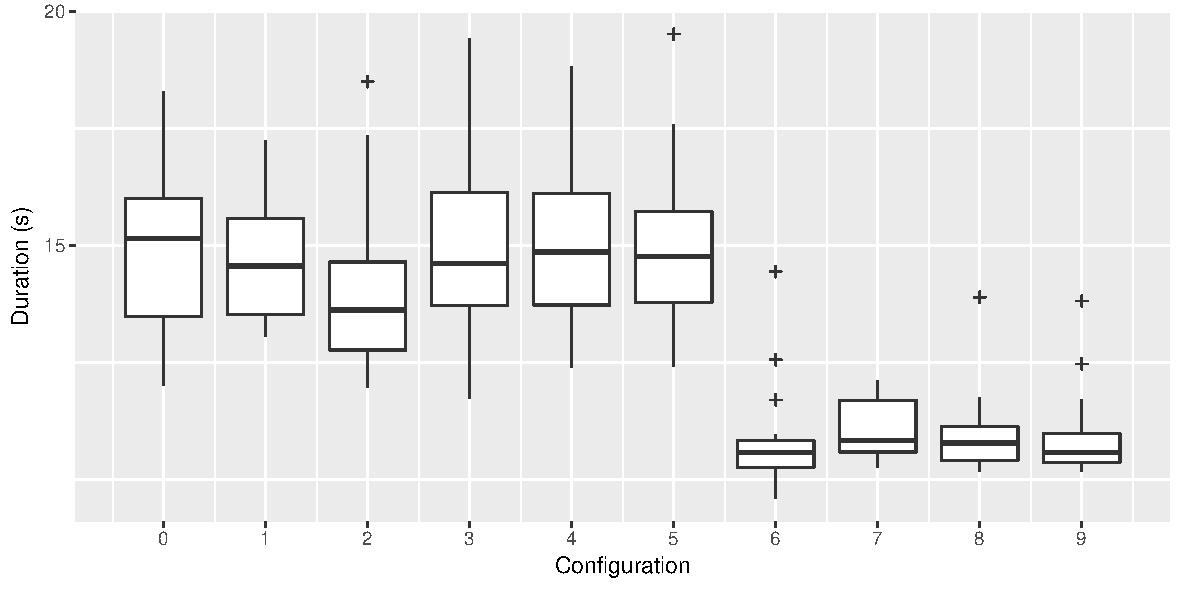
\includegraphics[width=\textwidth,keepaspectratio]{gfx/mean-durations-50k.pdf}
        \caption{50k}
        \label{fig:evaluation:performance:mean-durations-50k}
\end{figure}

\begin{figure}[htb]
        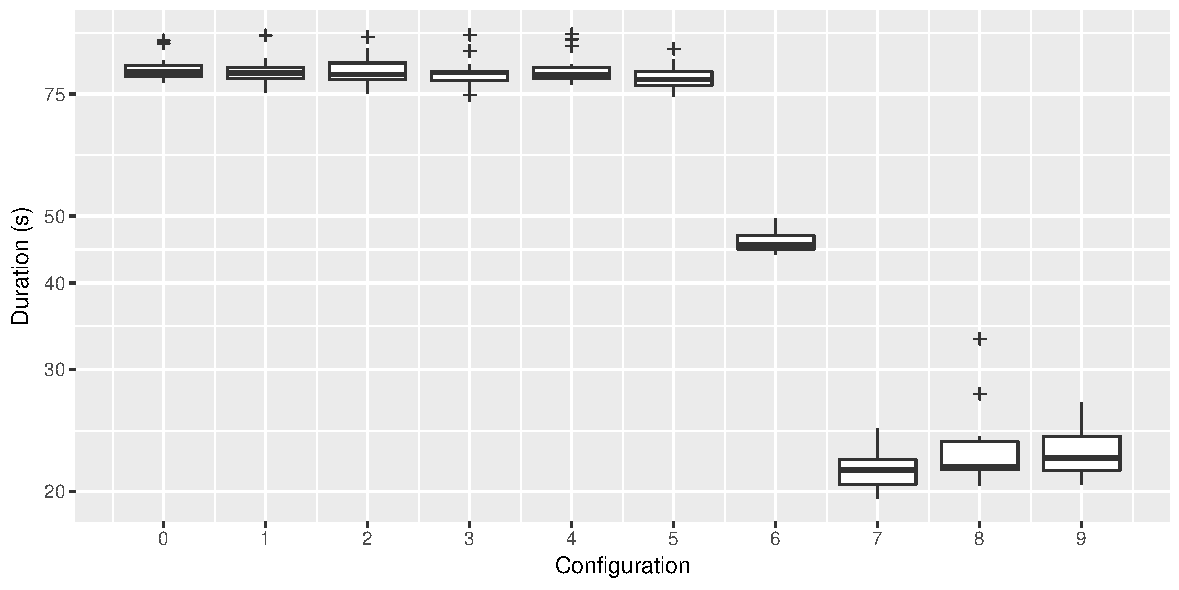
\includegraphics[width=\textwidth,keepaspectratio]{gfx/mean-durations-100k.pdf}
        \caption{100k}
        \label{fig:evaluation:performance:mean-durations-100k}
\end{figure}

\begin{figure}[htb]
        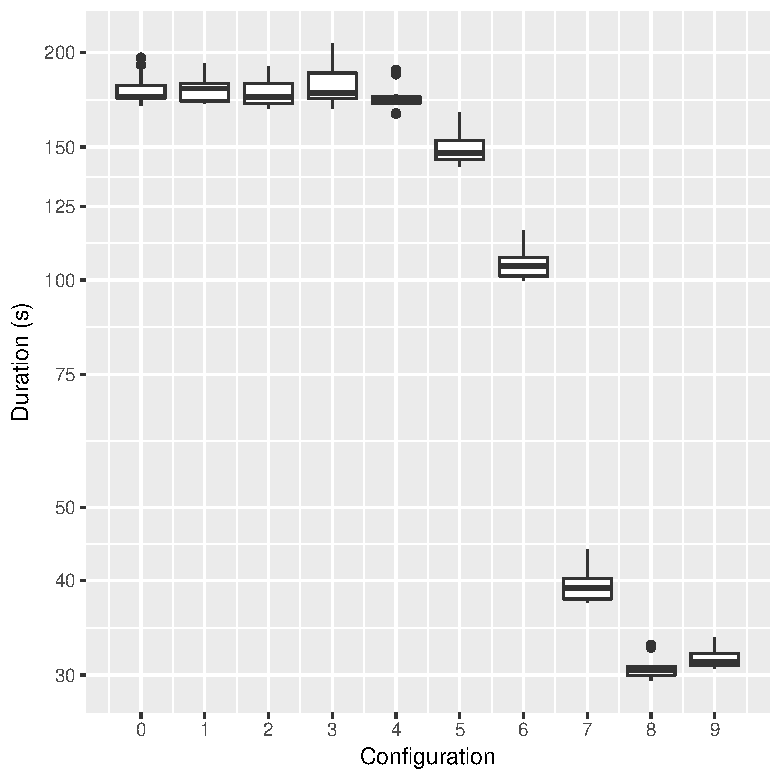
\includegraphics[width=\textwidth,keepaspectratio]{gfx/mean-durations-150k.pdf}
        \caption{150k}
        \label{fig:evaluation:performance:mean-durations-150k}
\end{figure}

\paragraph{Events over time}

The line plots in \cref{fig:evaluation:performance:config-comparison_50k,fig:evaluation:performance:config-comparison_100k,fig:evaluation:performance:config-comparison_150k} illustrate the amount of processed events over time for the respective experiment sizes.
These plots do not show a median or average distribution; instead, a specific experiment run was chosen that serves best for explaining the observations about the different configurations that were made earlier.

For each experiment size, the processed events over time are visualized in a separate line plot for each configuration, which are then merged in one figure.
The x-axes of all the plots indicates the time in seconds, while the y-axes indicate the amount of events that were processed and sent.
In this case, both axes use a continuous scale.
For improved visibility of patterns in the plots, an additional red line displays the smoothed conditional mean for each configuration.

When looking at the configurations for all experiment sizes and especially for the 100k and 150k experiments, it becomes apparent that for the lower configurations, the event processing rate drops low after a few seconds into the experiment.
This happens for configuration 5 and lower in the 50k experiment, for configuration 6 and lower in the 100k experiment and for configuration 7 and lower for the 150k experiment.
Thus, the more events have to be processed, the higher the buffer sizes and read batch size has to be in order to avoid this processing rate drop.

The earlier evaluation of the total processing duration already yielded the result that the configurations 0 to 5 perform poorly for all experiments.
When looking at the line plots, especially in \cref{fig:evaluation:performance:config-comparison_100k,fig:evaluation:performance:config-comparison_150k}, the reason for this becomes apparent:
Most of the time, the event processing rate at the bridge is extremely low, in some cases only 80 events were processed per second.
However, when the end of the subscription is near, the processing rate goes up dramatically -- even the lowest configuration peaks at over 6,000 events, a value which even the highest configuration never achieves in some runs.
It can additionally be observed that configurations 3 to 6 initially process a few thousand events per second, but afterwards the processing rate drops down low as well.
While the initial peak and subsequent dropdown can be explained by the computational complexity of managing the subscription, the peak near the respective goal remains mysterious.

The first thought was that a memory leak in the bridge application caused this behavior, but the fact that performance often suddenly increased again after about ten to twenty seconds made a memory leak very unlikely.
Inspection of the docker containers' resources via \texttt{docker stats} revealed that the single Event Store instance suffered heavy CPU load of up to 200\% (i.e. half of the CPU resources allocated to Docker).
Thus, the complexity of managing a persistent subscription and the resulting computation time was identified as a bottleneck.
An assumed possible solution for this was to make use of sharding in order to distribute the CPU load onto multiple Event Store instances.
While this would very likely still result in 200\% CPU usage, distributing the processing complexity onto multiple shards was expected to result in overall faster processing times for the bridge application.
In order to test this assumption, the experiment was repeated for 100,000 events and configuration 5, which shows a particularly strong occurence of this phenomenom.
As \cref{todo} shows, setting up an Event Store cluster does not improve performance of persistent subscriptions.
The assumption is that persistent subscriptions are managed by one shard only, maybe even only at the master shard, but this cannot be validated at this point.

%Instead, the messages per second rate was improved by tweaking several settings of the persistent subscription itself as well as the buffer size on the client side (i.e. the amount of messages per transaction that the client tells the server it can handle -- more buffer size means more messages per transaction, but could potentially overburden the client).

\begin{figure}[htb]
        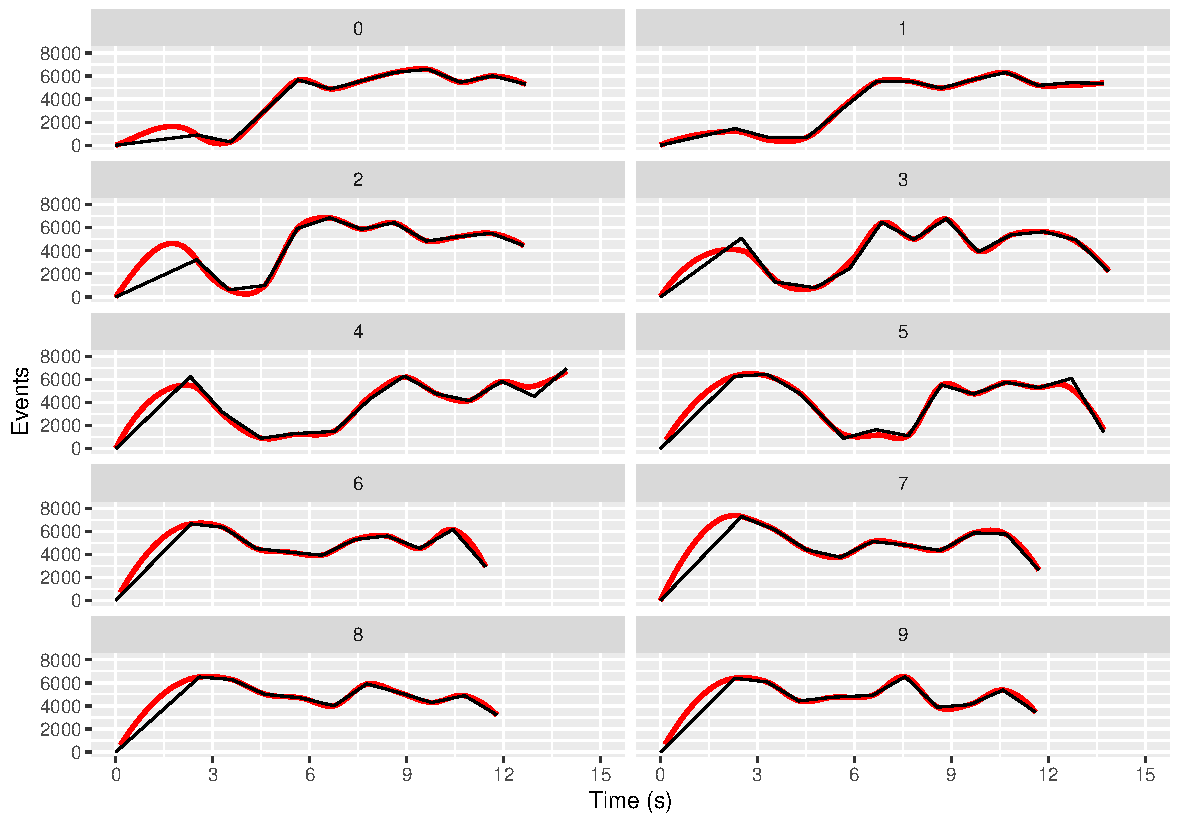
\includegraphics[width=\textwidth]{gfx/config-comparison_50k.pdf}
        \caption{50k}
        \label{fig:evaluation:performance:config-comparison_50k}
\end{figure}

\begin{figure}[htb]
        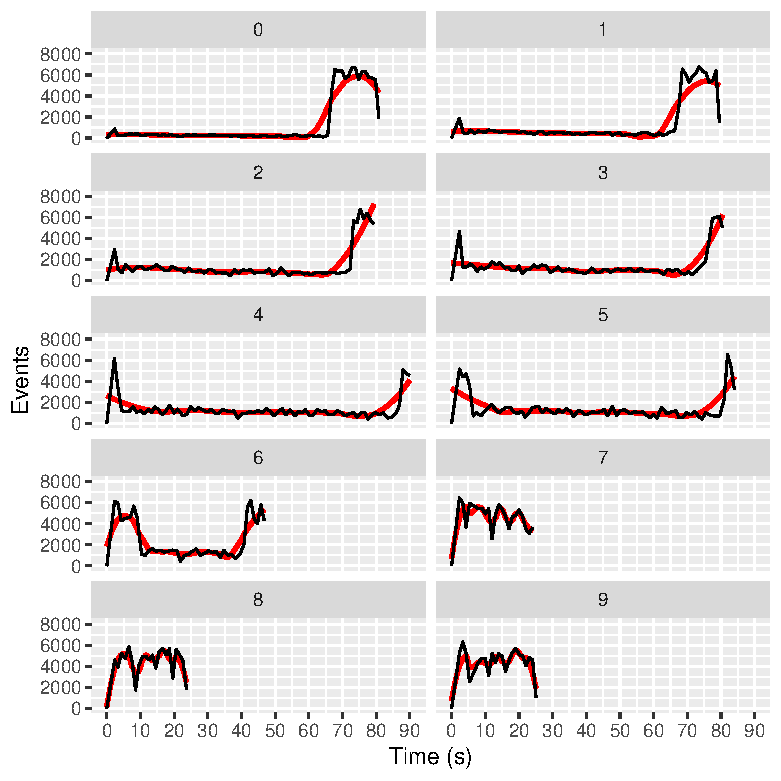
\includegraphics[width=\textwidth]{gfx/config-comparison_100k.pdf}
        \caption{100k}
        \label{fig:evaluation:performance:config-comparison_100k}
\end{figure}

\begin{figure}[htb]
        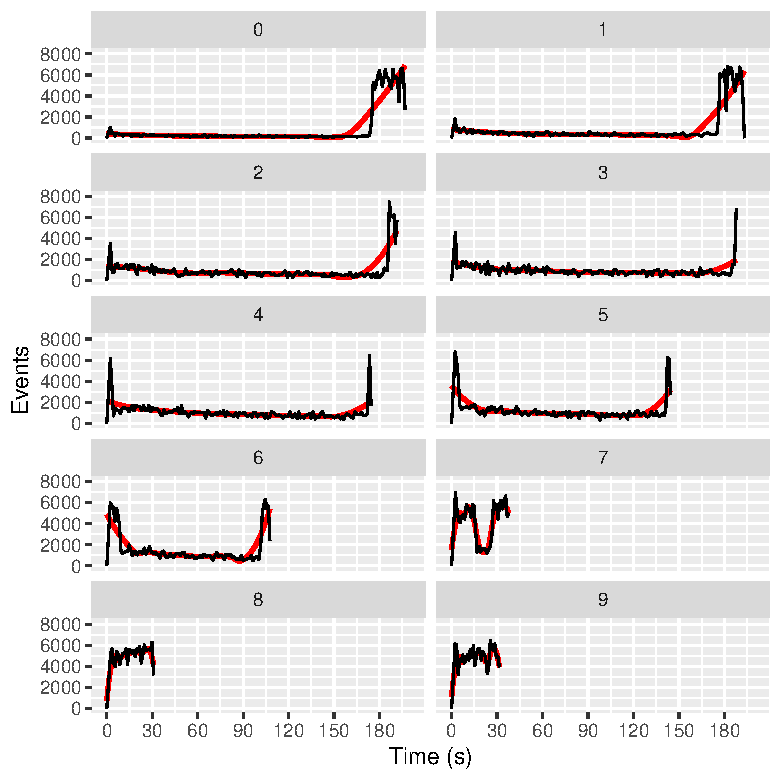
\includegraphics[width=\textwidth]{gfx/config-comparison_150k.pdf}
        \caption{150k}
        \label{fig:evaluation:performance:config-comparison_150k}
\end{figure}

While the experiments were running, Docker's ressources were manually monitored using the \texttt{docker stats} command.
The results are that the allocated ressources were sufficient for the experiments:
While cumulative CPU usage peaked at 300\%, i.e. three of the four possible threads were fully occupied, memory usage was rather low with about 1.5 GB for all containers.
As the resources that were made available to Docker were never fully used, it can be deducted that both CPU and memory were sufficiently high in order to not have a negative impact on the experiments.

\subsection{Elasticsearch Indexing Time}
\label{subsec:evaluation:performance:elasticsearch}

...

\subsubsection{Experiment Set-Up}

%In addition to the visualization statistics, the overall performance of the Elasticsearch cluster was monitored.
%Monitoring Elasticsearch cluster health out of the box is a feature of the X-Pack\footnote{\url{https://www.elastic.co/products/x-pack}} extension for the Elastic stack.
%X-Pack bundles various complementary capabilities such as security, reporting, and monitoring -- the latter of which could also be achieved manually via Elasticsearch's node stats API\footnote{\url{https://www.elastic.co/guide/en/elasticsearch/reference/current/cluster-nodes-stats.html}}.
%Although X-Pack is a commercial product, its basic license is free and the code is open source.
%Additionally, the monitoring feature from X-Pack that is used in this thesis, is merely used for evaluation purposes and thus \ac{IFAS} itself remains a combination of completely free and open sourced software products, without the need of registering for a license of any kind.

\subsubsection{Execution}

\subsubsection{Results}


\subsection{Elasticsearch to Kibana}
\label{subsec:evaluation:performance:kibana}

A separate test measures the performance of Kibana when visualizing large amounts of data.
For this purpose, 2,000,000 \texttt{ExperimentParticipated} events are created and forwarded to Elasticsearch.
Afterwards, a visualization of the experiment in Kibana -- similar to the A/B test visualization of the user test -- is then invoked which causes Kibana to poll the current state of the Elasticsearch index.
Kibana offers various statistics about its performance when rendering the visualizations, which are plotted in \cref{fig:evaluation:performance:}
As stated in \cref{sec:design:goals}, the total time from creation of the event to the event being displayed in its Kibana visualization should not be greater than 30 seconds.

\subsubsection{Experiment Set-Up}

\citet{Henze2011} collected 120,626,225 touch events in their experiment about touch performance of smartphone users, so if \ac{IFAS} is able to handle a similar number of events, it can be argued that the system's performance is adequate for performing testing and logging in general.
Thus, one variant of the performance test generates 150,000,000 events and pushes them -- via Event Store and the bridge -- through to Elasticsearch.
A number of metrics is recorded during this procedure:

\begin{description}
\item[Generation Duration] The amount of seconds it takes to generate all events and send a \ac{HTTP} POST request to the Event Store instance, enqueueing the event for saving.
\item[Event Store Save Duration] The amount of seconds it takes to save all events in the Event Store instance, beginning at the point in time where the first event is enqueued for saving.
\item[Elasticsearch Save Duration] The amount of seconds it takes to save all events in Elasticsearch, beginning at the point in time where the first document is enqueued for saving.
\item[Total Saving Duration] The amount of seconds it takes to save all events in \ac{IFAS}.
This value is similar to the Elasticsearch Save Duration, but takes into account the time it takes Event Store to process the first event and the bridge to forward the event to Elasticsearch.
Thus, the Total Saving Duaration also includes potential delays due to network latency when \ac{HTTP} requests are made.
As all Docker containers run in the same bridge network, the effect that this has on the Total Saving Duration is probably marginal.
\end{description}

As it is not realistic that 150,000,000 events are created nearly instantaneously -- in the referenced experiment~\cite{Henze2011} the events occurred over a timespan of a few months -- it is not required in this experiment to reach the 30s threshold mentioned earlier.
Instead, a number of smaller experiments is conducted in which the threshold has to be reached.
The performance test is thus repeated with the amount of generated events decreasing by one order of magnitude for each experiment (i.e. the experiment is performed with 15 / 150 / 1,500 / 15,000 / ... events).
For experiments with 150,000 events or lower, the 30s threshold of all data being available in Kibana has to be reached.
For the bigger experiments, this value is still monitored, but would not result in a failed experiment.
\todo{Change to 50k / 100k / 150k}

...\todo{how is this measured in ES/EvtS?}

Kibana offers the possibility to view detailed statistics for every visualization via the \emph{Visualization Spy}, including query duration, request duration and number of hits.
These statistics are useful for measuring the performance for different reasons:

\begin{description}
\item[Query Duration] This is the time Elasticsearch needed to complete process the query; it thus represents the time it takes Elasticsearch to handle the aggregation itself, without any networking overhead.\footnote{\url{https://discuss.elastic.co/t/what-is-query-duration-and-request-duration-in-kibana/50553}}
If the aggregation is complex, the query duration is usually high.
\item[Request Duration] In order to execute an aggregation and get its result, the request has to be sent to the Elasticsearch instance, which introduces additional overhead such as serializing and deserializing \ac{JSON} objects.
The request duration thus represents the duration from the point in time where Kibana decides to send the aggregation query, to the point where the results arrive in deserialized form back in Kibana.
As aggregation requests are usually of roughly the same size, the response can potentially contain a lot of complex data.
Thus, the request duration is a representation of how costly sending the data to Kibana is.
\item[Number of Hits] This represents the amount of documents that match the criteria given in the aggregation query.
As more data means more complex aggregation responses, this correlates with the request duration, but does not necessarily represent the complexity of the aggregation query.
For example, a query that matches all documents of an index would have a high number of hits, and a query matching only the document with index 1 would only have one hit -- but both queries are not complex and thus have a low query duration.
\end{description}

...

\subsubsection{Execution}

\subsubsection{Results}

\subsection{Combination of the results}
\label{subsec:evaluation:performance:insights}

It's fine.

In the end, the \emph{total visualization time} is calculated as follows:

$$t_\text{startES} - t_\text{startGen}+ d_\text{ESSave} + d_\text{VisDelay} + d_\text{VisRequest}$$

\todo{per Zeitstrahl oder so visualisieren}

\section{Null Hypothesis}

%short: what is the null hypothesis -- cf. \cite{Kohavi2009}
%\cite{Kohavi2013a}: To validate an experimentation system, we recommend that A/A tests be run regularly to test that the experimental setup and randomization mechanism is working properly. An A/A test, sometimes called a null test (Peterson 2004), exercises the experimentation system, assigning users to one of two groups, but exposes them to exactly the same experience.

% experimental set-up

% execution

% results

\section{Validity}
\label{sec:evaluation:validity}

\cite{Easterbrook2008a}: Construct, internal \& evernal validity, reliability

\section{Experimentation Guidelines for IFAS}

This section describes how different types of experiments can be executed using \ac{IFAS}.\todo{this is a kind of "subjective evaluation" -- maybe not the right place for this?}

\begin{description}
\item[A/B test]
\item[Null hypothesis] aka A/A test \cite{Kohavi2009}
\item[Collecting metrics] i.e. usage data in general, e.g. scroll time
\item[Collecting performance metrics(?)] (unclear, maybe into future work)
\item[Survey(?)] (maybe into future work, POC: Create user interview via \ac{IFAS})
\end{description}

 % INCLUDE: evaluation
% !TEX root = ../thesis-example.tex
%
\chapter{Conclusion}
\label{sec:conclusion}

\Blindtext[2][1]

\section{System Section 1}
\label{sec:conclusion:sec1}

\Blindtext[2][2]

\section{System Section 2}
\label{sec:conclusion:sec2}

\Blindtext[3][2]

\section{Future Work}
\label{sec:conclusion:future}

\Blindtext[2][2]
 % INCLUDE: future work
% !TEX root = ../thesis-example.tex
%
\chapter{Conclusion}
\label{sec:conclusion}

\Blindtext[2][1]

\section{System Section 1}
\label{sec:conclusion:sec1}

\Blindtext[2][2]

\section{System Section 2}
\label{sec:conclusion:sec2}

\Blindtext[3][2]

\section{Future Work}
\label{sec:conclusion:future}

\Blindtext[2][2]
 % INCLUDE: conclusion
\cleardoublepage

% --------------------------
% Back matter
% --------------------------
{%
\setstretch{1.1}
\renewcommand{\bibfont}{\normalfont\small}
\setlength{\biblabelsep}{0pt}
\setlength{\bibitemsep}{0.5\baselineskip plus 0.5\baselineskip}
\printbibliography[nottype=online]
\printbibliography[heading=subbibliography,title={Websites},type=online,prefixnumbers={@}]
}
\cleardoublepage

\listoffigures
\cleardoublepage

\listoftables
\cleardoublepage

% !TEX root = ../thesis.tex
%
\begin{appendices}
\label{ch:appendix}

\chapter{Source Code}
\label{ch:appendix:source}

\section{Docker}

\subsection{docker-compose.yml}

\lstinputlisting[label={appendix:code:docker:docker-compose},caption={docker-compose.yml}]{sourcecode/docker-compose.yml}

\end{appendices}
\cleardoublepage

% !TEX root = ../thesis-example.tex
%
%************************************************
% Declaration
%************************************************
\pdfbookmark[0]{Declaration}{Declaration}
\chapter*{Declaration}
\label{sec:declaration}
\thispagestyle{empty}

You can put your declaration here, to declare that you have completed your work solely and only with the help of the references you mentioned.

\bigskip

\noindent\textit{\thesisUniversityCity, \thesisDate}

\smallskip

\begin{flushright}
	\begin{minipage}{5cm}
		\rule{\textwidth}{1pt}
		\centering\thesisName
	\end{minipage}
\end{flushright}

%*****************************************
%*****************************************

\clearpage
\newpage
\mbox{}

% **************************************************
% End of Document CONTENT
% **************************************************
\end{document}
